%% 
%% Copyright 2007-2020 Elsevier Ltd
%% 
%% This file is part of the 'Elsarticle Bundle'.
%% ---------------------------------------------
%% It may be distributed under the conditions of the LaTeX Project Public
%% License, either version 1.2 of this license or (at your option) any
%% later version.  The latest version of this license is in
%%    http://www.latex-project.org/lppl.txt
%% and version 1.2 or later is part of all distributions of LaTeX
%% version 1999/12/01 or later.
%% The list of all files belonging to the 'Elsarticle Bundle' is
%% given in the file `manifest.txt'.
%% Template article for Elsevier's document class `elsarticle'
%% with numbered style bibliographic references
%% SP 2008/03/01
%% $Id: elsarticle-template-num.tex 190 2020-11-23 11:12:32Z rishi $
%\documentclass[preprint,12pt]{elsarticle}
% \documentclass[review,12pt, 3p, times]{elsarticle}
\documentclass[review,12pt, 3p, times]{elsarticle}
% review
% \documentclass[authoryear,preprint,review,12pt]{elsarticle}
%% Use the options 1p,twocolumn; 3p; 3p,twocolumn; 5p; or 5p,twocolumn
%% for a journal layout:
%% \documentclass[final,1p,times]{elsarticle}
%% \documentclass[final,1p,times,twocolumn]{elsarticle}
%% \documentclass[final,3p,times]{elsarticle}
%% \documentclass[final,3p,times,twocolumn]{elsarticle}
%% \documentclass[final,5p,times]{elsarticle}
%% \documentclass[final,5p,times,twocolumn]{elsarticle}
%% For including figures, graphicx.sty has been loaded in
%% elsarticle.cls. If you prefer to use the old commands
%% please give \usepackage{epsfig}
%% The amssymb package provides various useful mathematical symbols
\usepackage{amssymb}
\usepackage{graphicx}
\usepackage{longtable}
\usepackage{tipa}
\usepackage{cancel}
\usepackage{ulem}
\usepackage{pgf}
\usepackage{silence}
\usepackage{amssymb}
\usepackage{lineno}
\usepackage{enumitem}
\usepackage{lineno,hyperref}
\usepackage{natbib,stfloats}
\usepackage{multirow}
\usepackage{array}
\usepackage{multicol}
\usepackage{booktabs}
\usepackage{mathrsfs}
\usepackage{graphicx}
\usepackage{epstopdf}
\usepackage{latexsym}
\usepackage{mathtools}
\usepackage{algorithm}
\usepackage{algorithmic}
\usepackage{amsmath,amsfonts,amssymb}
\usepackage{rotating}
\usepackage{color}
\usepackage{colortbl}
\usepackage[caption=false]{subfig}
\usepackage[ruled,vlined,algo2e]{algorithm2e}
\usepackage{setspace}
\usepackage{tabularx}
\usepackage{xcolor}
\usepackage{adjustbox}
\usepackage{tikz}
\usepackage{pgf}
\usepackage{pgfplots}
\usepackage{pgfplotstable}
\usepackage{cancel}
\pgfplotsset{compat=1.3}
    \pgfplotstableread{
        0 0          -5.2
        1 0          -3.78
        2 0        20.16
        3 0        45.16
        4 0        19.68
        5 0        60.08
        6 0         15.99
        7 0         59.46
        8 0         -2.46
    }\dataset
\usepackage{setspace}
\usepackage{lineno}
\usepackage{pgfplots}
\pgfplotsset{/pgfplots/my legend/.style={
legend image code/.code={
\draw[dotted,thick,black](0cm,-0.01cm) -- (0.5cm,-0.01cm);%
   }
  }
}
\pgfplotsset{/pgfplots/my legend2/.style={
legend image code/.code={
\draw[dashed,thick,blue](0cm,-0.05cm) -- (0.5cm,-0.05cm);
   }
  }
}

%% \usepackage[authormarkup=none]{changes}
\usepackage[final]{changes}

\setlength {\marginparwidth }{2.1cm} 

\journal{International Journal of Production Economics}

\begin{document}
\begin{frontmatter}
\title{Incorporating Uncertain Human Behavior in Production Scheduling for Enhanced Productivity in Industry 5.0 Context }

\author[inst1]{Nourddine Bouaziz}
\author[inst2]{Belgacem Bettayeb}
\author[inst1]{M'hammed Sahnoun}
\author[inst3]{Adnan Yassine}

\affiliation[int1]{organization={CESI LINEACT},%Department and Organization
            addressline={80 avenue Edmund Halley}, 
            city={Saint-Étienne-du-Rouvray},
            postcode={76800}, 
            % state={State One},
            country={France}
            }
\affiliation[inst2]{organization={CESI LINEACT},
            addressline={8 Boulevard Louis XIV},
            postcode={59800},
            city={Lille},
            country={France}
            }
\affiliation[inst3]{organization={LAMH, Le Havre University Normandy},
            addressline={25, rue Philippe Lebon},
            postcode={76600},
            addressline={Le Havre},
            country={France}
            }








\begin{abstract}
 
\replaced[comment]{ Human-centered }{ Human-centred }production systems are of increasing interest \replaced[comment]{ to }{ for } researchers, especially with the advent of the Industry 5.0 paradigm. Most research into production scheduling has long neglected \replaced[]{ human workers' }{ the } specific roles and unpredictable \replaced[comment]{behavior }{ behaviour of human workers } in a production system, treating them as machines with deterministic \replaced[comment]{ behavior}{ behaviour }. This work studies the impact of human operational \replaced[comment]{ behavior }{ behaviour }on the performance of a production system and proposes an optimization model to allocate workers' profiles to\replaced[comment]{ workstations}{ machines}. We modeled the punctuality profile as a Markov chain representing a worker's productive and non-productive states. We developed a simulation process based on \added[comment]{the} multi-agent system (MAS) paradigm to test the effectiveness of the proposed model and to measure the impact of workers' behaviors and their assignments to different workstations on the productivity of the workshop. A non-linear programming model is also proposed to provide the optimal assignment of workers to \replaced[comment]{ workstations }{ machines } while maximizing the throughput of a \replaced[comment]{ dual-resource-constrained }{ dual-resource constrained } flow-shop production system for a given mix of production. The results obtained highlight the significant impact of human operator behavior on the performance of a production system. The findings demonstrate the importance of incorporating human behavior models into the decision-making process for assigning workers to workstations based on their operational profiles.
\end{abstract}


\begin{keyword} 
Human behavior \sep Markov Chain Modeling \sep Worker Assignment   \sep Production Scheduling \sep Nonlinear Optimization \sep Simulation 


\end{keyword}
\end{frontmatter}

\section{Introduction}
Over the past decade, the emergence of Industry 4.0 has heralded a new era in industrial practices. Industry 4.0 has paved the way for \replaced[comment]{ developing }{ the development of } smarter and self-sufficient \replaced[comment]{ systems by seamlessly integrating digital technologies with physical }{ By seamlessly integrating digital technologies with physical systems, } systems. However, this transformation requires human operators to adapt to the production systems~\cite{lyngstadaas2022harder,fantini2020placing,pinzone2020framework}. This industrial revolution has been driven by \replaced[comment]{}{  a focus on } improving profitability through increased product and/or service quality and process efficiency, achieved through various digital technologies~\cite{raja2023industry}. As a result, the manufacturing industry has undergone a significant transformation due to digitalization. It has invented new organizational and managerial methods at all product life cycle stages, from product design to its disposal~\citep{messaadia2016plm}. This revolution is founded on \replaced[comment]{}{the principles of } data collection, analysis, and intelligent decision-making\added[comment]{ principles}, made possible by \deleted[comment]{ a suite of } cutting-edge technologies such as big data, sensors, cloud computing, and cyber-physical systems \citep{brik2022fog}. It allows \replaced[]{  the acquisition of }{ gaining }{}  more knowledge about production tools, processes, and their interaction with human operators \cite{kadir2020human}. In any industry, accurate knowledge of human behavior provides a significant advantage in predicting future system states and optimizing decision-making at the strategic, tactical, and operational levels \citep{bailly2020}. Therefore,\replaced[comment]{ although }{ even though }Industry 4.0 has introduced innovative technologies that improve production efficiency, new challenges have emerged\replaced[comment]{}{ rapidly}, focusing on issues such as human well-being, sustainability, and resilience \citep{lyngstadaas2022harder}.
\\ 
The industrial sector has increasingly depended on automatic machines to perform repetitive, precise, and/or low-value-added tasks. However, recent studies have shown that \replaced[comment]{successfully integrating }{  the successful integration } technologies with human workers is crucial to \replaced[comment]{ realizing }{realize }their full potential benefits~\citep{chen2022analysis,kose2023game,dolgui2022design}. Along with other technical factors, the interaction between humans, smart tools, and management systems plays a critical role. It must be considered and modeled at the operational management level of these heterogeneous systems. 
\added[comment=$R1^{4}$]{Furthermore, industrial organizations face a dual challenge, as they must deal with both low attractiveness and high turnover rates \cite{Jamal2019Work}. Despite being the cornerstone of economies worldwide, these sectors struggle to retain skilled talent, hindering their growth and stability. Research indicates that classical production systems, which impose numerous rules on workers, stifle worker innovation and elevate turnover levels \cite{Acar2018Creativity}.}
For these organizations, ensuring optimal productivity, workplace safety, and high levels of worker motivation is imperative.  
\\
As a result, there is a justified, almost urgent, shift towards Industry 5.0, which seeks to address the shortcomings of Industry 4.0. The ultimate goal is to use technologies intelligently, placing humans at the forefront of the system while being mindful of the sustainability of the planet~\cite {Destouet2023,battini2022towards}. \added[]{The human-centric aspect of Industry 5.0 can be ensured through various means, including prioritizing human involvement in the decision-making process, fostering collaborative working methods, and implementing intelligent and tailored scheduling systems.} 

\added[comment=$R1^{4}$]{This paper delves into the development of human-centric production scheduling, where organizations endeavor to adapt systems to align with human behavior. }
\added[comment]{The objective of this work is twofold. First, we aim to prove the benefit of integrating a model of human behavior into the decision-making process of a dual-resource-constrained scheduling problem to reduce the impact of potential performance-degrading events resulting from such behavior. Secondly, our goal is to propose a mathematical model able to provide an optimal allocation of workers of different profiles to machines while maximizing the throughput of the production system in a fixed time frame. This work's main contributions include:}
\begin{itemize}
    \item \added[comment]{Development of a multi-agent-based simulation model integrating Markov chain-based modeling of human behavior profiles.}
    \item \added[comment]{Simulation-based demonstration of the importance of the composition of behavior profiles (homogeneous and heterogeneous) of workers in enhancing the performance of the production system while respecting human nature.}
    \item \added[comment]{Development of a non-linear optimization model that considers various heterogeneous behavioral profiles of workers.}
    \item \added[comment]{Implementation and comparison of two optimization methods for worker allocation to machines: simulation-based and non-linear programming optimization.} 
\end{itemize}


\added[comment]{
The rest of the article is structured as follows. Section~\ref{sec:litreview} provides a comprehensive literature review encompassing various perspectives on how human behavior is approached within the industry. Section~\ref{sec:approach1} details the approach adopted to model and simulate human behavior and shows its impact on the productivity of a dual-resource-constrained flow-shop production system. The first step of the proposed approach, the modeling and simulation of human behavior, is presented with its results in Section~\ref{sec:res1}. The mathematical model proposed for optimizing the scheduling problem that incorporates human behavior is detailed in Section~\ref{sec:Pre_mod}. Then, Section~\ref{sec:Exp_dis} focuses on experimentation and discussion of the results. Section~\ref{sec:mins} highlights some managerial insights from the results. Finally, Section~\ref{sec:conc3} presents the main conclusions and perspectives of this work.
}
\section{\added[comment=$R1^{1}$]{Literature review}}\label{sec:litreview}
\added[comment=$R1^{1}$]{To explore the literature on human behavior modeling and integration in the industry, we based our research on the Scopus database, followed by Google Scholar research to include some additional work from the snowball effect. We used the following keywords for the initial article selection queries: ``Industry 5.0", ``human-centered", ``dual-resource production system," ``human behavior modeling," ``stochastic human behavior modeling," and ``worker assignment problem." In this literature review, we first explored the human-centric aspect of Industry 5.0, the modeling of human behavior, and the importance of taking such models into account. We focused later on dual-resource production systems and work assignment problems, which allowed us to position our contribution among a list of articles addressing the incorporation of human factors into production systems optimization.} 

% keyworks : Uncertain human behavior - Production scheduling - Industry 5.0 -  Productivity - Human-machine interaction - Markov Chain Modeling  - Worker Assignment - Nonlinear Optimization 
%  - Simulation

Industry 5.0, a concept coined by the European Commission,\replaced[comment]{ focuses }{ places a special focus } on the essential role of human operators. Unlike Industry 4.0, this shift emphasizes the importance of humans in the industrial environment~\cite{battini2022towards}. Highly advanced technological systems, such as s, smart buildings and complex organizational structures, work \replaced[comment]{ with humans to accomplish }{ together with humans to carry out } repetitive and strenuous tasks. This collaboration is intended to promote not only  economic and environmental sustainability \replaced[comment]{, but also }{ and resilience  a }social sustainability that contributes significantly to the \replaced[comment]{ company's resilience }{ resilience of the company } \cite{missimer2017strategic}. This can be ensured by providing workforce development initiatives and keeping the central place of humans in industry, which leads to a robust and efficient workforce. Tasks that require creativity and perception-based skills remain in the domain of humans, creating a partnership or connection between humans and intelligent technology. A more complete review \replaced[]{of }{ about } social sustainability can be found in \cite{trost2022social}.

Consequently, human behavior modeling will play a pivotal role in Industry 5.0, continuing to attract the attention of \replaced[comment]{  social science and humanities }{ in social science and humanities, as well as } researchers and industrial engineers~\citep{panagou2023scoping}.
For example, in human-robot collaboration, \citep{zanchettin2018} proposed a technique to predict human activity patterns. This approach enables \deleted[]{a} quick identification of when \added[comment]{  the human will require a } particular collaborative operation\replaced[comment]{}{ will be required by the human}, thereby allowing a robot \replaced[]{to perform other autonomous functions simultaneously}{ to simultaneously perform other autonomous functions}. The prediction algorithm uses a higher-order Markov chain (with memory) and was tested in a scenario involving a dual-arm robot used for a collaborative assembly task of small parts. In their study, \citep{zhang2021task} explored the scheduling of tasks for a collaborative robotic assembly cell to strike a balance between the work cycle and human fatigue. For a more comprehensive overview of the latest research on human-robot interactions in the industrial sector, the reader can refer to \citep{hjorth2022human, liu2022application, vicentini2021collaborative, hentout2019human}.
	
Recognizing the critical role that the human factor plays in modern industrial systems, \replaced[comment]{ much }{ many } research \replaced[comment]{ is }{ are } currently involved in modeling and simulating human behavior to improve human well-being at work and to prevent possible negative effects of certain behaviors on system performance in terms of cost, quality, and safety \citep{Jahanmahin2022}.
Thus, since human behavior is influenced by several exogenous parameters dependent on the surrounding context, different considerations for modeling human behavior can be found in the literature in several domains:  i) ergonomics \citep{ferjani2015,ferjani2017, Berlin2017, Greig2019}, ii) human reliability \citep{Azarkhil2014,DiPasquale2013,Dantan2020}, iii) cybersecurity \citep{Upadhyay2022,SanchezAguayo2021,Domarkiene2021,Moallem2021} and iv), and industry \citep{Schia2019,Kong2020,Mossa2015}. In a recent survey paper on the consideration of workers’ differences in production systems \replaced[comment]{ modeling }{ modelling }and design ~\cite{Katiraee2021a}, the authors reported that 74\% of the selected works deal with the problem of assignment of work. 

Based on ~\cite{Katiraee2021a}, and after adding filters and the snowball approach of the selected articles, we summarise in Table~\ref{tab:researchcomparison} the most relevant studies that address the problem of work assignment that include a specific aspect of human behavior, such as skill level, efficiency, or punctuality. The comparison of the work presented in Table~\ref{tab:researchcomparison} reveals that 86\% of the \replaced[comment]{}{  presented } papers address the worker assignment problem. Among them, only two papers (\cite{ayough2023robust} and \cite{Bouaziz2022}) consider the stochastic aspect of human behavior. In general, only four works properly consider the uncertain behavior of humans in industrial systems. 
Regarding the methods used, approximately 48\% of the papers use metaheuristics and 52\% use exact methods. There are 24\% of papers that deploy both resolution approaches simultaneously.
\replaced[comment]{ Only 14\% utilize simulation, }{ Concerning simulation, only 14\% utilize this approach, } despite its powerful contributions to representing uncertain behavior. Human behavior is considered differently in each work. Among the explored research works,\added[comment]{ the }skill level is \replaced[comment]{ considered in 61\% of articles, capability in 14\%, flexibility in 10\%, and punctuality in 14\%. }{ taking into account in 61\% of them, capability in 14\%, } 
It should be noted that \replaced[comment]{  only one of }{ among } the articles dealing with punctuality\replaced[comment]{}{, only one } aimed to improve the system through simulation; the others did not consider any optimization approach to enhance the production system. 
Recent literature reviews have underscored the significance of scheduling problems that incorporate human operators, including the work of Dhiflaoui et al. \cite{dhiflaoui2018dual} \replaced[]{, which }{that} presents a comprehensive survey of dual source constants and \replaced[comment]{ classifies }{classify}  existing research. The authors emphasize the need \replaced[comment]{ to develop }{ for developing }  more realistic models. More recently, Geurtsen et al. \cite{geurtsen2023production} \replaced[]{examined }{ examine } several research endeavors \replaced[comment]{ to integrate }{centered on integrating} workers into scheduling problems. Additionally, Battini et al. \cite{battini2022towards} provide an intriguing literature review on job rotation scheduling considering human factors.\replaced[comment]{ They identify }{  identifying }scheduling as a key aspect of  Industry 5.0's human-centric approach, which emphasizes the importance of considering human factors in the design and operation of manufacturing systems. Hashemi et al. \cite{hashemi2020operations} offer an insightful overview of papers dealing with dual resource problems and highlight the importance of prioritizing the realistic scheduling of human operators.
% In Table~\ref{tab:researchcomparison}, we review the most relevant studies that address the problem of work assignment and a specific aspect of human behavior, such as skill level, efficiency, or punctuality.
	
In the industrial domain, \citep{Bogataj2018,Onay2023,Bentefouet2012} notice that \deleted[comment]{ the } human \replaced[comment]{ behavior }{ behaviour } needs to be more explicitly considered in scheduling models. However, most of the scheduling models presented in research have only considered the skill aspect of human \replaced[comment]{ behavior }{ behaviour } and \replaced[comment]{ analyzed }{ analysed } how it \replaced[comment]{ affects }{ effects } the performance of production systems. 
\cite{lucchese2023stochastic} confirms that \added[]{given} the complex and uncertain \replaced[]{behavior}{behavoir} of a human worker, it seem\added[]{s} appropriate to model such behaviors as stochastic processes to rationalize their study and analysis. However,\replaced[comment]{ limited }{ few }  research \replaced[comment]{ has }{ have } embedded the stochastic aspect of human \replaced[]{behavior}{behavoir} in the modeling of socio-technical systems. For instance,  \citep{lin2022human} proposed a hidden \replaced[comment]{ semi-Markov  }{ semiMarkov  } model (HSMM) to model human \replaced[comment]{ behavior }{ behaviour } in production systems. The applicability of the proposed model has been validated by simulation.
\citep{vijayakumar2022framework} proposes a new framework that integrate the human factor into production and logistics systems. It combines different levels of decision-making to improve performance, quality, and well-being.
To take into account social relationships between workers, \citep{elkosantini2009integration} developed a Markov chain-based worker \replaced[comment]{ behavior }{ behaviour } model. The results highlighted the impact of such relationships on individual performance.

The Markov chain paradigm is also used in \citep{chang2008synthesized} to model customer profiles based on the ERG (Existence, Relatedness, Growth) theory. Proposed in 1969  by Alderfer, the ERG theory emphasizes the needs of individuals in a hierarchical order. This theory is based on Maslow's work, which reduced the number of needs to three levels. However, the ERG theory differs from Maslow's in three ways: (i) it allows for multiple levels to be pursued at the same time; (ii) it allows for different orders of needs for different people; and (iii) if the highest level of needs remains unsatisfied, a person may regress to a lower level of needs that are more easily fulfilled, with the hierarchy of needs represented by states. In this context, the different states of the Markov chain correspond to different levels or categories of customer needs. The transition probabilities between states reflect the likelihood of customers moving from one need category to another over time. By \replaced[comment]{ analyzing }{ analysing } observed transitions and estimating transition probabilities, the Markov chain model can provide information on customer \replaced[comment]{ behavior }{ behaviour } and the dynamics of their needs. Even if this approach is \replaced[comment]{ modeling  }{ modelling  } an important aspect of human \replaced[comment]{ behavior}{ behaviour }, it seems not applicable directly in a workshop environment, at least due to the difference in the time scale. However, the use of \added[]{ the } Markov chain demonstrates its flexibility and efficiency in the \replaced[comment]{ modeling  }{ modelling  } of human \replaced[comment]{ behavior}{ behaviour }.  

Therefore, accurate \replaced[comment]{ behavioral }{  behavioural } models of production resources are essential to optimize the production system and \replaced[comment]{ minimize }{ minimise }its operating cost. These models can be very useful in static and dynamic production planning and scheduling to anticipate and reduce the effect of operational hazards caused by the fortuitous \replaced[comment]{ behavior }{ behaviour } of these resources, which is the case with human operators. Moreover, such models are also essential for predicting the \replaced[comment]{ behavior }{ behaviour } of the system as a whole and its ability to adapt to and overcome external disturbances.

Through their review of the literature, \citep{Jahanmahin2022} found that most research work developing models of human \replaced[comment]{ behavior }{ behaviour } in the industrial or social environment uses simulation\replaced[comment]{, e.g. }{ex.} \citep{Digiesi2009}, or real systems to validate their models. 
Although the human being has often been taken into account in the various operations management models in the literature, especially regarding the deterministic components of \replaced[comment]{human's behavior}{ his behaviour }, such as fatigue \cite{ferjani2017,Digiesi2009}, efficiency in performing tasks \cite{BERTI2021108151,digiesi2020human}, and experience\cite{korytkowski2017competences}. Few recent works propose stochastic models to represent human behavior. For example, Lucchese et al. \cite{lucchese2023stochastic} model the processing time of each worker with a normal distribution, while Ayough et al. \cite{ayough2023robust} consider the diverse stochastic skills of workers. An aspect often overlooked in research is the recognition that human behavior and performance can vary significantly from one worker to another, with particular attention to the unpredictable nature of human behavior, including punctuality during work. 
\deleted[comment]{
The objective of this work is twofold. First, we aim to prove the benefit of integrating a model of human \replaced[comment]{ behavior }{ behaviour } into the decision-making process of a dual-resource-constrained scheduling problem to reduce the impact of potential performance-degrading events resulting from such \replaced[comment]{ behavior}{ behaviour }. Secondly, our goal is to propose a mathematical model able to provide an optimal allocation of workers of different profiles to machines while maximizing the throughput of the production system in a fixed time frame. This work's main contributions include:}
% \begin{itemize}
%     \item \deleted[comment]{Development of a multi-agent-based simulation model integrating Markov chain-based modelling of human \replaced[comment]{ behavior }{ behaviour } profiles.}
%     \item \deleted[comment]{ Simulation-based demonstration of the importance of the composition of \replaced[comment]{ behavior }{ behaviour } Profiles (homogeneous and heterogeneous) of workers in enhancing the performance of the production system, while respecting human nature.}
%     \item \deleted[comment]{Development of a non-linear optimization model that considers various heterogeneous behavioral profiles of workers.}
%     \item \deleted[comment]{Implementation and comparison of two optimization methods for worker allocation to machines: simulation-based and non-linear programming optimization.}
% \end{itemize}

Table~\ref{tab:researchcomparison} compares our contribution to other works considering the human factor in industry. It \added[comment]{highlights how our solution} is the sole contribution \added[comment]{to} addressing the punctuality problem with a stochastic approach and using \replaced[]{an }{ the} exact method of resolution and simulation \added[comment]{techniques}.

\begin{table}[H]
    \centering
    \adjustbox{width=\textwidth}{
	\begin{tabular}{c|ccccccccc}
		\hline
            %    &  & & \multicolumn{3}{c}{\added[]{Resolution method}} & \\
		\added[]{Ref.}          & Worker Assignment         & Stochastic & (Meta-)heuristic & Exact method & Simulation & Aspect \\ 
                \hline
			\citep{Al-E-Hashem2009} & \checkmark &            &                & \checkmark   &            & Skill levels     \\ 
			\citep{Chu2019}      & \checkmark &            &      \checkmark          &              &            & Skill levels                   \\ 
   \citep{green2017hybrid}     &            &            &                &              & \checkmark & Skill levels            \\
			\citep{Mura2019a}       & \checkmark &            & \checkmark     &              &            & Skill levels                    \\ 
			\citep{Mura2019b}     & \checkmark &            & \checkmark     &              &            & Skill levels                    \\ 
			\citep{Ramezanian2015}  & \checkmark &            & \checkmark     &              &            & Skill levels                   \\ 
			\citep{ferjani2017}     & \checkmark &            & \checkmark     &              & \checkmark & Skill levels           \\ 
			\citep{Liu2019}         & \checkmark &            &                & \checkmark   &            & Skill levels           \\ 
			\citep{Chen2019a}      & \checkmark &            & \checkmark     & \checkmark   &            & Skill levels        \\ 
			\citep{Katiraee2022}    & \checkmark &            &                & \checkmark   &            & Skill levels         \\ 
			\citep{Wu2018a}      & \checkmark &            & \checkmark     & \checkmark   &            & Skill levels                   \\ 
			\citep{Zacharia2015}     & \checkmark &            & \checkmark     &              &            & Skill levels                   \\
   \citep{ayough2023robust}  & \checkmark  & \checkmark& & \checkmark & & Skill levels \\
			\citep{Borba2013}  & \checkmark &            & \checkmark     & \checkmark   &            & Capability \\ 
			\citep{Vila2014}    & \checkmark &            &                & \checkmark   &            & Capability  \\ 
			\citep{Moussavi2017} & \checkmark &            & \checkmark     & \checkmark   &            & Capability           \\ 
   			\citep{LUO2023102534}   & \checkmark &            & \checkmark     &      \checkmark        &            & Flexibility                   \\ 
      \citep{li2023integrating}  & \checkmark & & & \checkmark  & &Flexibility\\
      \citep{Lundstrom2016}   &            & \checkmark &                &              &            & Punctuality                   \\ 
			\citep{Sanchez2020}   &            & \checkmark &                &              &            & Punctuality                   \\ 
   	\citep{Bouaziz2022}   & \checkmark  & \checkmark  &                &                      & \checkmark & punctuality            \\
		\hline 
				\textbf{This work }    & \textbf{\checkmark } & \textbf{\checkmark } &                & \textbf{\checkmark } & \textbf{\checkmark } & \textbf{punctuality}             \\ \hline

		\end{tabular}
	}
 \caption{Summary of research work considering \replaced[comment]{humans}{human} in industry. \added[comment]{It considered the following comparison indicators: \textbf{Worker Assignment:} The consideration of the worker assignment problem; \textbf{Stochastic:} Some parameters of the considered models are stochastic; \textbf{(Meta-)heuristic and Exact method:} The nature of the resolution method; \textbf{Simulation:} A simulation approach is used to solve the problem; \textbf{Aspect:} The aspect considered in human modeling} }
 \label{tab:researchcomparison}
\end{table}

\deleted[]{ The rest of the article is structured as follows. Section~\ref{sec:approach1} details the approach adopted to model and simulate human \replaced[comment]{ behavior }{ behaviour } and shows its impact on the productivity of a dual-resource constrained flow-shop production system. The first step of the proposed approach, the modeling, and simulation of human behavior, is presented with its results in Section~\ref{sec:res1}. The mathematical model proposed for the optimization of scheduling problem that incorporates human \replaced[comment]{ behavior }{ behaviour } is detailed in Section~\ref{sec:Pre_mod}. Then, Section~\ref{sec:Exp_dis} focuses on experimentation and discussion of the results.\replaced[]{ Section }{The section}\ref{sec:mins} gives some managerial insights highlighted from the obtained results. Finally, Section~\ref{sec:conc3} presents the main conclusions and perspectives associated with this work.}

\section{Proposed approach }\label{sec:approach1}
To effectively examine the correlation between human \replaced[comment]{ behavior }{ behaviour } and productivity and subsequently improve the assignment of workers to \replaced[comment]{ workstations}{ machines }, we perform the process illustrated in Figure~\ref{fig:approach}. 
A dual resource flow-shop production system is considered, where a machine and a human operator are required to execute any task. Unlike traditional flow shops relying solely on machines, this model introduces workforce availability as an additional constraint. This dual resource constraint is a major challenge in scheduling tasks in this type of workshop, and the versatility of workers complicates it even further. In addition to machine availability and capabilities,\replaced[comment]{ the }{  } scheduler must consider worker availability and skills \cite{dhiflaoui2018dual}. We chose this production system as \added[]{an} application because even \added[]{though} it has been extensively studied, it remains a system rich \replaced[comment]{ in }{ of }  challenging \replaced[comment]{ problems }{ problem } \cite{elkosantini2009integration, dhiflaoui2018dual}. It also aligns with Industry 5.0 by involving human behavior modulation, a key challenge \cite{battini2022towards}. Hybrid human-machine systems offer flexibility and cost benefits but introduce scheduling difficulties due to dynamic interactions and optimizing mixed resource allocation \cite{elkosantini2009integration,costa2020solving}.

In the first phase, the \replaced[comment]{ behavior }{ behaviour } of human operators is \replaced[]{modeled}{modelled} using a Markov chain whose states represent the different places an operator can be in the workshop.
Different and diverse behavioral profiles of workers are affected by various factors (such as fatigue, experience,  age, etc.), which we aggregate into a single factor observed through a Markov model reflecting the changes in productivity states of each profile. These worker profiles are classified according to their productivity state, which is directly linked to their physical location on the production floor. To model these states, a Markov chain is used, delimiting 'productive zones' (PZs), e.g., workstations, where workers actively contribute to \added[]{the} production, and `non-productive zones' (NPZs), e.g., the cafeteria, where their activities do not contribute to productivity. This approach makes it possible to represent, and \replaced[]{analyze }{ analyse } how workers move from one state to the other, providing insight into their productivity patterns and spatial \replaced[comment]{ behavior }{ behaviour } within the workspace. The variability within NPZs lies in the likelihood of workers remaining in these zones, which influences the length of their stay. For example, in zones such as smoking \replaced[]{ zones }{zone}, individuals have a variety of \replaced[]{behaviors}{ behaviours}: some refrain from smoking, others smoke occasionally, and still others smoke frequently. These \replaced[]{behaviors}{ behaviours} represent the distributions of visit frequencies, departure frequencies, and lengths of stay in the NPZ.
We do not assume that there is a specific zone that is particularly more attractive than others for all \replaced[]{ profiles }{ profile }, but that each profile may have its own more attractive NPZ.
Concerning the impact on productivity, the NPZ that degrades it the most is also different from one profile to another because it will have the highest value of average stay time weighted by visiting frequency.


Using the Markov chain \replaced[comment]{ behavior }{ behaviour } model, the second phase consists of two methods to optimize the allocation of operators to workstations.
The first method uses a simulation approach based on a multi-agent system (MAS) architecture, and the second method consists of solving a non-linear programming optimization model.
The third phase contains the test and comparison of the two methods.
	
\begin{figure}[h!]
	\centering
	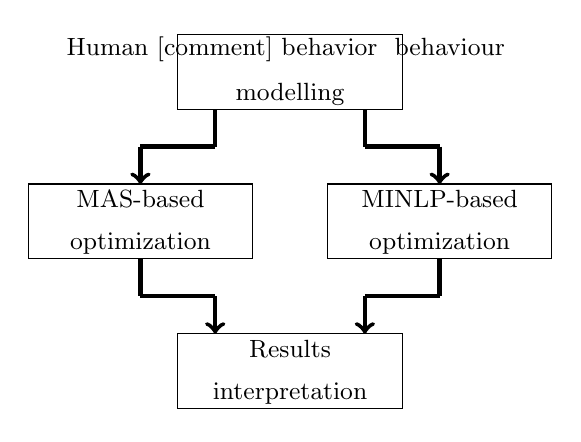
\begin{tikzpicture}[scale=0.95]
		\draw[ draw = black, fill=white](-1.5,9) rectangle (1.5,8);
		\draw (0,8.8) node{\small Human \replaced[comment]{ behavior }{ behaviour } };
		\draw (0,8.2) node{\small modelling};
		\draw [draw = black, -, ultra thick] (-1,8) -- (-1,7.5);
		\draw [draw = black, -, ultra thick] (-1,7.5) -- (-2,7.5);
		\draw [draw = black, ->, ultra thick] (-2,7.5) -- (-2,7);
		\draw [draw = black, -, ultra thick] (1,8) -- (1,7.5);
		\draw [draw = black, -, ultra thick] (1,7.5) -- (2,7.5);
		\draw [draw = black, ->, ultra thick] (2,7.5) -- (2,7);
		\draw[draw = black, fill=white] (-3.5,7) rectangle (-0.5,6);
		\draw (-2,6.8) node{\small MAS-based };
		\draw (-2,6.2) node{\small optimization};
															        
		\draw [draw = black, -, ultra thick] (-2,6) -- (-2,5.5);
		\draw [draw = black, -, ultra thick] (-2,5.5) -- (-1,5.5);
		\draw [draw = black, ->, ultra thick] (-1,5.5) -- (-1,5);
															        
		\draw[draw = black, fill=white] (0.5,7) rectangle (3.5,6);
		\draw (2,6.8) node{\small MINLP-based };
		\draw (2,6.2) node{\small optimization};
		\draw [draw = black, -, ultra thick] (2,6) -- (2,5.5);
		\draw [draw = black, -, ultra thick] (2,5.5) -- (1,5.5);
		\draw [draw = black, ->, ultra thick] (1,5.5) -- (1,5);
		\draw[draw = black, fill=white] (-1.5,5) rectangle (1.5,4);
		\draw (0,4.8) node{\small Results };
		\draw (0,4.2) node{\small interpretation};
	\end{tikzpicture}\\	
	\caption{The proposed approach}
	\label{fig:approach}
\end{figure}
	
\subsection{Simulation method}\label{sec:res1}
\subsubsection{MAS model}
To investigate and quantify the impact of human behavior on production system productivity, we developed a multi-agent system (MAS) based simulator. The MAS comprises autonomous agents representing different elements of the real system, interacting with each other. Three interconnected agents, namely “Worker", “Job", and “Zone", make up the simulator (see Figure~\ref{fig:interaction}). Each agent's composition and role are defined as follows: 
\begin{itemize}
    \item Worker: \replaced[comment]{this agent }{ it } interacts with all other agents because a worker executes a job  \replaced[comment=$R1^{3}$]{ while being at }{ when he is on } a workstation and moves between zones (productive or non-productive).\added[comment=$R1^{12}$]{ It is important to note that a worker's presence in an NPZ area can sometimes be unrelated to their behavior but caused by an unexpected external event (e.g., injury caused by a machine or a safety device failure). This is why we model it using stochastic parameters to accurately characterize its frequency and duration. }The worker's parameters are:
    \begin{itemize}
        \item \textit{Last\_zone}: contains the index of the last zone visited by the worker before updating his location.
	\item \textit{Profile}: the movement patterns of workers between productive and non-productive zones are encapsulated within worker
        profiles, which are represented by a transition probability matrix -Markov chains-. This matrix defines the probabilities of movement between zones based on predefined profiles, which may vary among individual workers.  
        \item \textit{Next\_zone}: index of the next zone to be visited by the worker.
        \item \textit{Methods}: \replaced[]{  }{ the role of the agent worker} is to operate the product on the workstation when he is present and the product is ready. \deleted[]{This agent moves from zone to zone } \replaced[]{A}{a}ccording to the Markov chain model associated with his behavioral profile, this agent moves from zone to zone.  
    \end{itemize} 
    \item Zone: this agent is a reactive agent representing workstations (WS) and non-productive zones (NPZ) located in the workshop. Each 'zone' agent is characterized by the following:
    \begin{itemize}
        \item\textit{Type}: classifies the zone as \textit{productive} (a workstation) or \textit{non-productive} (e.g., infirmary, restaurant, etc.)
        \begin{itemize}
            \item \added[comment=$R1^{2}$]{Productive zone, known as the workstation, constitutes the working environment for employees. Each workstation may consist of simple or complex tools and machinery, with the expectation that they can be operated by a single human worker}
            \item \added[comment=$R1^{2}$]{non-productive zone: encompasses all areas where the operator is not actively engaged in work, such as break rooms, restaurants, smoking areas, and similar spaces.}
        \end{itemize}
        
        \item\textit{Status}: status of the zone, which may be  \textit{free} or \textit{occupied}. 
    \end{itemize}
    \item Job: this agent represents the products \added[]{(jobs)} that workers need to process as each product passes through all workstations on the production floor. Each job is characterized by the following parameters:
    \begin{itemize}
        \item\textit{\replaced[]{LastWS}{Index}}: the current or last workstation visited by the “Job" agent (product)
	\item\textit{PT}: a list of processing times at each required workstation when the worker is present
    \end{itemize}
\end{itemize}		      			
\begin{figure}[htbp]
	\centering
	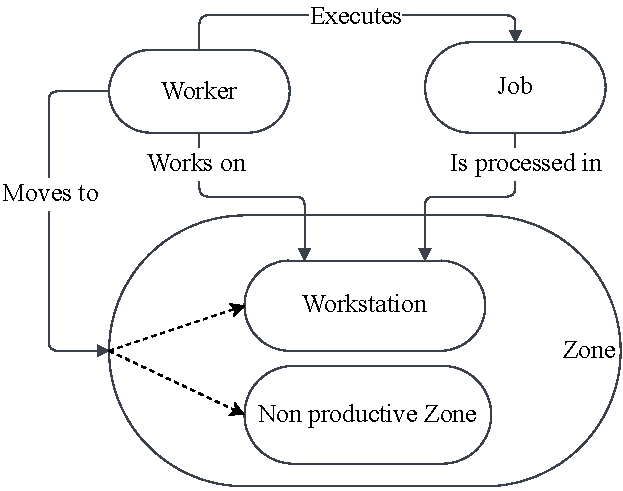
\includegraphics[trim=00 00 00 00, clip, width=7cm]{AgentsInteractions.pdf}
	\caption{Multi-agent model's agents and their interactions}
	
	\label{fig:interaction}
\end{figure}
	
\subsubsection{System and human behavior modeling}
We consider the following production system composed of a set of $M$ workstations (WS) denoted by $\mathcal{W\!S}=\{W\!S_m, m=1,2,..,M\}$ associated with a set of workers (WK) denoted by $\mathcal{W\!K}=\{W\!K_k, k=1,2,..,K\}$.
Each workstation corresponds to a machine that needs the presence of a worker while processing a task. Each job (product) is automatically transferred to the subsequent required workstation until it completes all the necessary processing steps. Let $PT$ be the vector representing the processing times of all workstations:  
$PT=[PT_1,.., PT_m,.., PT_M]$  and let $AP$ be the vector representing the assigned workers with different \replaced[comment]{ behavior }{ behaviour } profiles to workstations: $AP=[AP_1, ..., AP_k, ..., AP_K]$. 
In addition to workstations, we also define a set of $Z$ zones within the workshop where workers can go and stay for a while, making their workstation and the task that is performed on standby until they return. These zones are called “non-productive zones" (NPZ) and are denoted by $\mathcal{NPZ}=\{N\!P\!Z_z, z=1,2,..,Z\}$. The NPZ represents the areas where a worker is in a state of non-productive activity, such as a break, personal call, lunch, or simply an unjustified absence from the workstation.

Since a worker's next state (zone and action) primarily depends on their current state, \replaced[comment=R]{it is}{it's} possible to model their behavior as a Markov process, which is a powerful mathematical tool for representing stochastic and uncertain phenomena. We model the behavior of workers using a classical Markov chain of $Z+1$ states that correspond to the possible locations where a worker can go and stay. For each worker, the possible states (locations) belong to two classes: i) one of the $M$ ``productive" states, which corresponds to the workstation to which the worker is assigned ($p_{11}^k$), and ii) $Z$ ``non-productive" states that correspond to the NPZ (see Figure~\ref{fig:states}).

\begin{figure}[h]
	\centering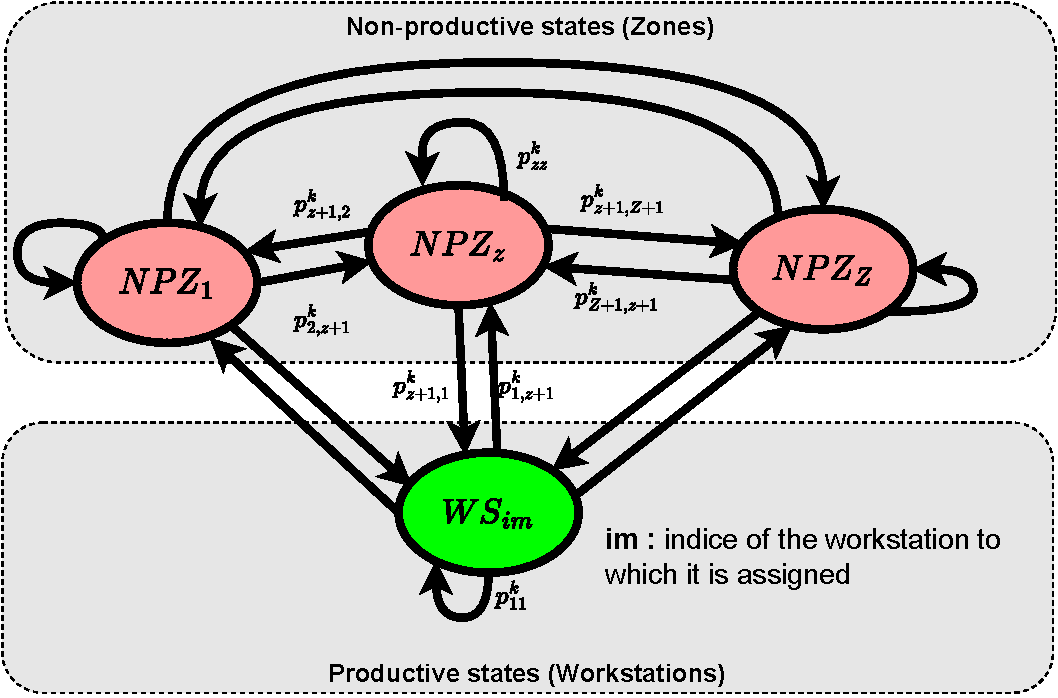
\includegraphics[ clip, width=0.5\linewidth]{markovModel.pdf}

 \caption{Productive and non-productive States of Markovian-Based Human \replaced[comment]{ Behavior }{ behaviour } Model}
	\label{fig:states}
\end{figure}
We assume that each worker is assigned to a unique workstation, which does not change during the time horizon considered\replaced[comment=$R1^{3}$]{. Workers }{, and that he } can only move back and forth between \replaced[comment=$R1^{3}$]{ their designated }{ this } workstation and the set of NPZ. The transition probabilities between each workstation and the non-productive zones are defined by the transition matrix $P^k$ relative to the $k^{th}$ generic profile of workers' \replaced[]{behaviors }{ behaviours}.
\begin{equation}\label{eq:tmatrix}
	P^k_m =
	\left( {\begin{array}{ccccccc}
		p_{11}^k & p_{12}^k & p_{13}^k & \dots & p_{1z'}^k & \dots &p_{1(Z+1)}^k\\
		p_{21}^k & p_{22}^k & p_{23}^k & \dots & p_{2z'}^k & \dots &p_{2(Z+1)}^k\\
		p_{31}^k & p_{32}^k & p_{33}^k & \dots & p_{3z'}^k & \dots &p_{3(Z+1)}^k\\
		\vdots & \vdots & \vdots & \ddots & \vdots & \ddots & \vdots\\
		p_{z1}^k & p_{z2}^k & p_{z3}^k & \dots & p_{zz'}^k & \dots &p_{z(Z+1)}^k\\
		\vdots   & \vdots &\vdots & \ddots & \vdots & \ddots &\vdots\\
		p_{(Z+1)1}^k & p_{(Z+1)2}^k & p_{(Z+1)3}^k & \dots & p_{(Z+1)z'}^k & \dots &p_{(Z+1)(Z+1)}^k\\
		\end{array} } \right)
\end{equation}

As shown in Equation (\ref{eq:tmatrix}), ($p_{11}^k$) represents the probability that a worker with profile $k$ will remain at the workstation to which he/she is assigned, let's say $\textit{WS}_m$, $p_{1z}^k, \forall z\in \{2,.., Z+1\}$ represents the probability that a worker with profile $k$ moves from workstation $\textit{WS}_m$ to a non-productive zone $\textit{NPZ}_z$, $p_{z1}^k$ represents the probability that a worker moves back from a non-productive $\textit{NPZ}_z$ to his workstation $\textit{WS}_m$, and $p_{zz'}^k, \forall z,z'\in \{2,..., Z+1\} $ represents the probability of moving from $\textit{NPZ}_{z}$ to $\textit{NPZ}_{z'}$.
	
\subsubsection{Simulation procedure}
The algorithm deployed is presented in Algorithm~\ref{algo:algorithmsimulator}. When the simulation starts, three variables are initialized to zero: the simulation clock \textit{tick}, the number of completed jobs \textit{NFJ}, and the effective processing times of jobs on \replaced[comment]{ workstations }{ machines } \textit{EPT}$_{jm}$. The state of the entire system is updated at each new tick until the \added[]{end of the} fixed time horizon. To update the status of all agents at each time step (tick), a specific process is followed.
First, all workstations are activated, and their availability \replaced[]{ as well as }{ and } associated workers and operations within the input buffers $InB_{k}$ are assessed. Once these conditions are met, the value of the variable $EPT_{jm}$ increases. If $EPT_{jm}$ is equal to $PT_{m}$, it indicates that the job has been completed on the workstation $\textit{WS}_m$. The job is then moved to the input buffer $InB_{k+1}$ if the current workstation is not $\textit{WS}_K$. However, if the current workstation is $\textit{WS}_K$, the completed job $j$ is transferred to the output buffer $OutB$ of that workstation (last workstation). If the current workstation is $\textit{WS}_1$, a new job is generated. 

During this process, the worker is not present all the time on his workstation but follows the Markovian process to move between the productive zone (his workstation) and non-productive zones (break, nursery, lunch). These zones serve as an example used to model various reasons for worker absence from the workstation. \added[comment=$R1^{5}$]{The workstation is not productive when the worker is absent.} In this model, the production operations can be interrupted when the transition to a new position is generated by the Markov chain model.


\begin{algorithm2e}[H]  
\algsetup{linenosize=\tiny}
  \scriptsize
	\KwData{}	 
	\ \ $\mathcal{WK}=\{WK_1, WK_2,.., WK_K\}$: Set of workers\;
	\ \ $\mathcal{WS}=\{WS_1,WS_2,..,WS_M\}$: Set of workstations\;
	\ \ $\mathcal{J}=\{1,..,J\}$: Set of jobs indices\;
	\ \ $\mathcal{K}=\{1,..,K\}$: Set of workers' (workstations) indices\;
	\ \ $PT=(PT_{m}:  m\in\mathcal{M})$: Processing times vector\;
	\ \ $InB=(InB_m: m\in\mathcal{M})$: Workstations' input buffers\;
	\ \ $OutB$: Output buffer of completed jobs (buffer of the last workstation)\;
	\ \ $Horizon$: Simulation horizon\;
	\ \  $EPT_{jm}$: the effective processing time of the job $j$ on the Workstation $m$\;
	\ \ $tick$: unit of time that passes between iterations of the simulation \;
	\KwResult{}
	\ \ \it{NFJ}: Number of finished jobs  \; 
	\ \ $Productivity$: Productivity rate  \;
	\Begin{
		Initialization: $tick=1$ , \quad  \it{NFJ}$=0$ , \quad  \it{EPT}$_{jm}=0 \quad  \forall j\in\mathcal{J} \  \forall m\in\{1,..,M\}$\;
		\While{$tick <= Horizon$}{
			
			Update workers' locations\;
			\For{Each  $Ws_m\in\mathcal{WS}$}{
   \For{Each  $WK_k\in\mathcal{WK}$}{
				\If{($Ws_m$ is occupied by $j\in\mathcal{J}$ \textbf{AND} $WK_k$ is present) \textbf{OR} ($Ws_m$ NOT occupied \textbf{AND} \ $\exists j\in\mathcal{J}$ in $InB_m$ \textbf{AND} $WK_m$ is present)}{
					$EPT_{jm}  \leftarrow	  EPT_{jm}+1$ \; 
					\If{$EPT_{jm} = PT_{jm}$ }{
						\eIf{$m =M$ }{
							Transfer job $j$ to $OutB$ \;
							$NFJ \leftarrow NFJ+1$\;
						}
						{
							Transfer job $j$ to $InB_{m+1}$\;
							\If{m=1}{
								Generate a new job at $Ws_1$
							}
						} 
					}
				}
			}}
        $tick\leftarrow tick+1$\;		
  }
		$Productivity\leftarrow \frac{NFJ}{Horizon}$\;
	}
	\caption{Simulation algorithm}
            \label{algo:algorithmsimulator}
\end{algorithm2e}	   
				
\subsection{Optimization model}\label{sec:Pre_mod}
In this section, we introduce our non-linear optimization model designed to identify the most efficient worker-to-machine assignment, ultimately \replaced[comment]{ maximizing }{ maximising } productivity for the \replaced[comment]{ dual-resource-constrained }{ dual-resource constrained } flow-shop production system. 
The principle assumptions of our model are the following:
\begin{enumerate}
    \item  The time required to move a product between two successive \replaced[comment]{ workstations }{ machines } is negligible 
    \item No setup time is required to switch between product types on all \replaced[comment]{ workstations }{ machines } 
    \item Each \replaced[comment]{ workstation }{ machine } is assigned only one worker \added[comment=$R1^{6}$]{ and each worker is assigned to at most one workstation }. 
    \item Once a worker is assigned to a \replaced[comment]{ workstation}{ machine }, their assignment remains unchanged throughout the entire scheduling period
    \item The number of workers available is equal to or greater than the number of \replaced[comment]{ workstations }{ machines }
    \item Operations can be interrupted without incurring any additional time to restart them.
\end{enumerate}

\subsubsection{Notations}
\begin{longtable}{p{.08\textwidth} p{.92\textwidth}}
    \hline
    \multicolumn{2}{c}{Sets }\\
    \hline
    $\mathcal{M}$ & set of workstations (productive zones), with $|\mathcal{M}|=M$                      \\
    $\mathcal{T}$ & set of  product types	with $|\mathcal{T}|=T$\\
    $\mathcal{K}$ & set of workers, with $|\mathcal{K}|=K$\\
    $\mathcal{P}$ & set of worker profiles available on the job market, with $|\mathcal{F}|=P$\\
    \hline
    \multicolumn{2}{c}{Indices }\\
    \hline
    $m$           & indices of workstations, with $m\in\{1,2,..,M\}$\\
    $j$           & indices of jobs, with $j\in\{1,2,..,J\}$\\
    $t$           & indices of job types (product) , with $t\in\{1,2,..,T\}$\\
    $k$           & indices of workers, with $k\in\{1,2,..,K\}$\\
    $p$           & indices of profiles, with $p\in\{0,1,2,..,P-1\}$\\
    \hline
    \multicolumn{2}{c}{Parameters}\\
    \hline
    $H$           & time horizon of production                                 \\
    $I$           & production mix, with $I=(I_1,I_2,..,I_t,..,I_T)$ where $I_t$ is the minimum demand for the type of product $t$ .\\
    $f_{k,p}$     & a binary variable indicating whether the worker $k$  belongs to the profile $p$, where each worker can get only one profile $\sum_{p\in\mathcal{P}} f_{p,k} =1  \quad\forall k\in\mathcal{K}$\\
    $\lambda^1_p$ & average duration of the working time period of the workers of the profile $p$\\
    $\lambda^0_p$ & average duration of the absence time period of the workers of the profile $p$\\
    $\tau_{t,m}$  & reference processing time of the product type $t$ on workstation $m$\\
    $\alpha_k$    & average continuous working time of the worker $k$\\
    $\gamma_k$    & average absence time of the worker $k$ after a period of working time\\
    $J$           & the maximum number of products (all types combined) that can be produced:\\
	           & $J=\displaystyle\max_{t\in{\cal T}}\left\lceil {(H-\sum_{m\in\mathcal{M}} \tau_{t,m})}/{\max_{m\in\mathcal{M}} \tau_{t,m}}\right\rceil$, where $\left\lceil x    \right\rceil $   is the smallest integer greater than or equal to $x$ \\
    $HV$          & a \replaced[]{ high-value }{ high value } number\\
    \hline
    \multicolumn{2}{c}{Decision variables }\\
    \hline		
    $X_{t,j}$     & a binary variable indicating if the $j$-th job is a product of type $t$ \\
    $Y_j$         & a binary variable indicating the launch of the $j$-th job, i.e. equals 1 if the product is assigned to a product type, 0 otherwise: $Y_j = {\sum_{t\in \mathcal{T}} X_{t,j}} \quad\forall{j \in\mathcal{J} }$ \\
    $W_{k,m}$     & a binary variable indicating if the worker $k$ is assigned to the workstation $m$\\
    $N_{j,m}$     & the number of interruptions (due to the absence of worker) to the job $j$ on workstation  $m$\\
    $U_m$         & the average continuous productivity time (up-time) of the workstation $m$:\\ 
                  & $U_m=\sum_{k\in \mathcal{K}} \alpha_k \times W_{k,m} \quad \forall{ m \in  \mathcal{M}}$\\
    $D_m$         & the average \replaced[]{continuous }{ continues } non-productivity time (downtime) of the workstation $m$: \\
                  & $D_m = \sum_{k\in\mathcal{K}} \gamma_k \times W_{k,m} \quad\forall m\in\mathcal{M}$\\
    $\Pi_{j,m}$   & the effective processing time of the job $j$ at the machine $m$. It includes the real processing time and the absence time of the operator:\\
	           & $\Pi_{1,m} = N_{1,m}\times D_m  + \sum_{t\in\mathcal{T}} ( X_{t,1} \times\tau_{t,m}) \quad \forall m\in\mathcal{M} $\\
	             & $\Pi_{j,m} =  (N_{j,m}-N_{j-1,m})\times D_m + \sum_{t\in \mathcal{T}}(X_{t,j} \times \tau_{t,m})\quad\forall{j=2..J} \quad  \forall m\in\mathcal{M}$\\
    $C_{j,m}$     & the completion time of the job $j$ on workstation  $m$\\
    $\Pi^C_{j,m}$ & the cumulative processing time to the job $j$ at the machine $m$\\
	             & $\Pi^C_{1,m} = \sum_{t\in \mathcal{T}} (X_{t,1} \times\tau_{t,m})\quad\forall m \in\mathcal{M}$\\
	             & $\Pi^C_{j,m} =\Pi^C_{j-1,m} +  \sum_{t\in \mathcal{T}} (X_{t,j} \times \tau_{t,m} ) \quad\forall j=2..J \quad\forall m \in\mathcal{M}$  \\							
    \hline
\end{longtable}		
	
\begin{figure}[htbp]
	\centering
	\rotatebox{0}{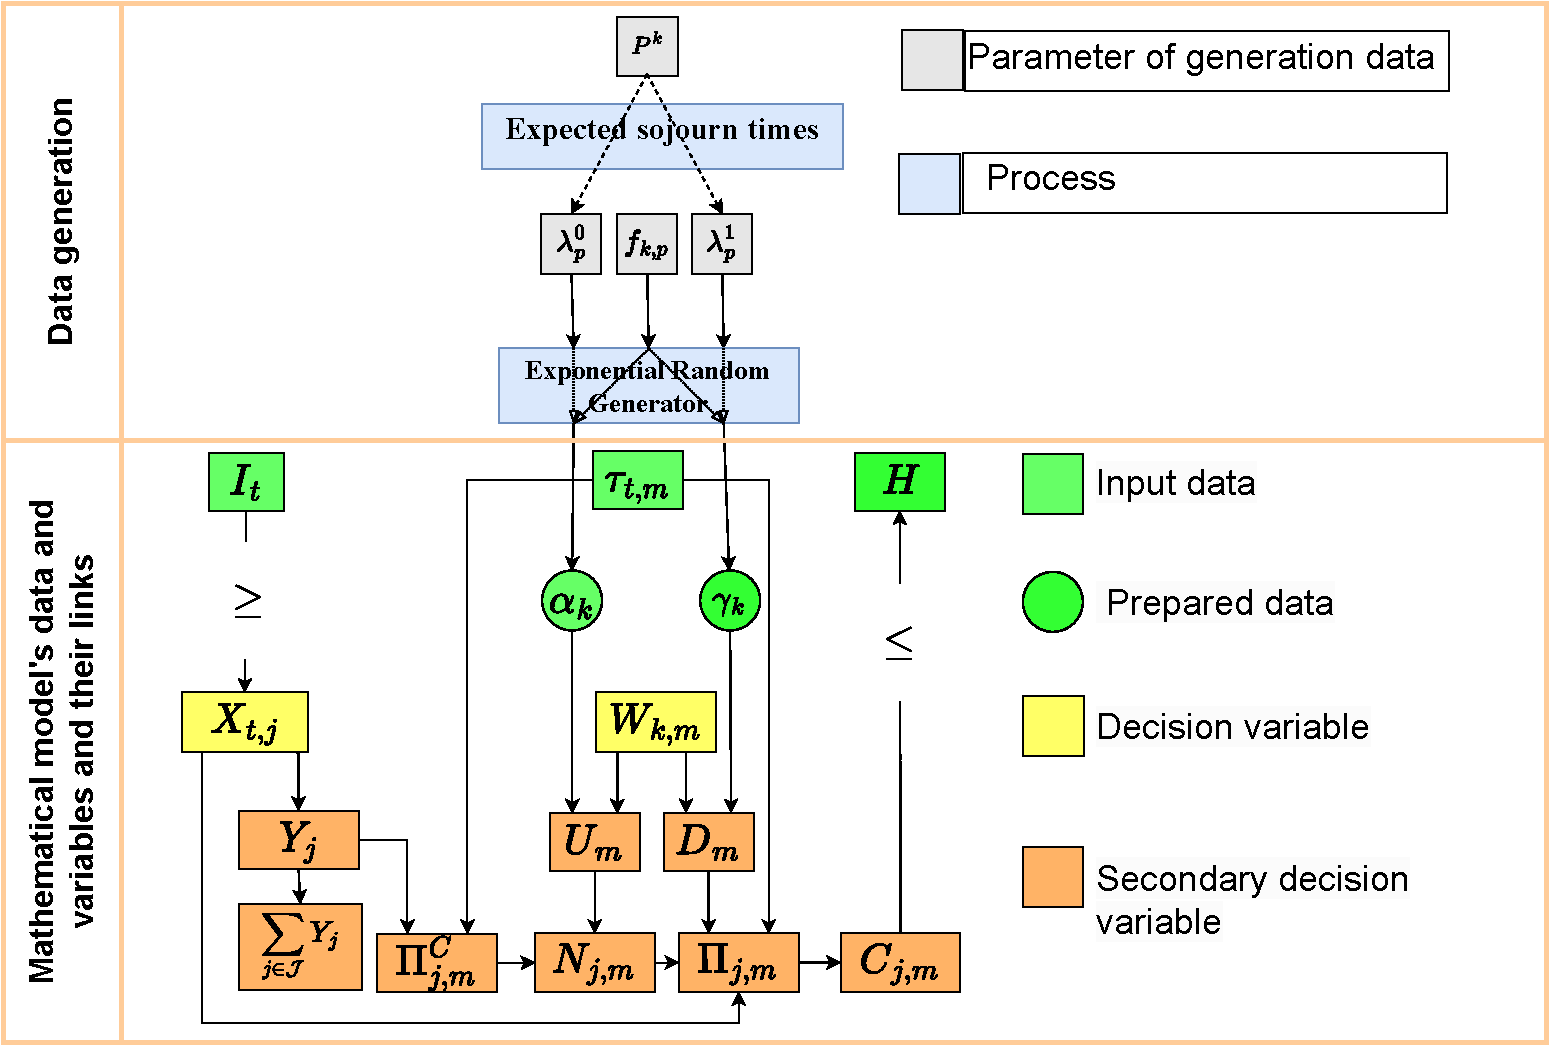
\includegraphics[width=12cm]{ModelVariablesLinks.pdf}}
	\caption{Mathematical model's data and variables and their links}
	\label{fig:ModelVariablesLinks2}
\end{figure}
					
					              
\subsubsection{Problem formulation}
The \replaced[comment]{ dual-resource-constrained }{ dual-resource constrained } flow-shop production system worker assignment and scheduling problem \replaced[]{are formalized }{is formalised } by \added[]{ the }Mixed Integer Nonlinear Programming  model:
\begin{equation}
	\text{{\it obj}: Maximize } \sum_{j=1..J}Y_j\label{obj1}
\end{equation} 		
The objective of our model is to maximize the productivity of the production system across a finite time horizon for all types of products. Therefore, the objective function in Eq.~(\ref{obj1}) aims to Maximize the total number of finished products during the considered time horizon. Alternatively, the objective function could be to \replaced[]{ minimize }{ minimise } the makespan of a given number of demanded products. However, we choose to Maximize the throughput to facilitate comparison with the simulation part and obtain a stable comparison between different scenarios.
	
This objective function is subject to the following constraints:
\begin{spacing}{.5}	
	\begin{equation}
		\begin{array}{ll}		
			  &   
		\end{array}
		{{\sum_{k\in \mathcal{K}}W_{k,m}}=1 \quad \forall{ m \in  \mathcal{M}}}
		\label{c3}
	\end{equation}
	\begin{equation}
		\begin{array}{ll}
			  &   
		\end{array}
		{{\sum_{m\in \mathcal{M}}W_{k,m}}\leq 1 \quad \forall{ k \in  \mathcal{K}}}
		\label{c4}
	\end{equation}
	% \begin{equation}\label{c5}
	% {\color{red}   	X_{t,j}  \leq 1  \quad\forall j \in \{1,...,J\}\quad\forall{t\in\mathcal{T}}}
	% \end{equation} 
	\begin{equation}\label{c6}
		X_{t,j}  \leq I_t  \quad\forall j \in \{1,...,J\} \quad \quad\forall{t\in\mathcal{T}}
	\end{equation} 
	\begin{equation}\label{c7}
		{{\sum_{j=1..J} X_{t,j} }   \geq I_t   \quad \quad\forall{t\in\mathcal{T}}}
	\end{equation} 
	\begin{equation}\label{c8}
		\text{\quad }  Y_j\leq Y_{j-1} \quad\forall j \in \{2,...,J\}
	\end{equation}									 
	\begin{equation}\label{c9} 
		N_{j,m} +1 \geq \frac{\Pi^C_{j,m}}{U_m}  \quad\forall j \in \{1,...,J\}  \quad\forall m\in\mathcal{M}
	\end{equation}
											
	\begin{equation}\label{c10} 
		N_{j,m}  + 0.001  \leq \frac{\Pi^C_{j,m}}{U_m}  \quad\forall j \in \{1,...,J\} \quad\forall m\in\mathcal{M}
	\end{equation}
											 
	\begin{equation}\label{c11}
		C_{1,1} = \Pi_{1,1} 
	\end{equation}
																				
	\begin{equation}\label{c12}
		C_{j,m} \geq Y_j\times\Pi_{j,m}+C_{j-1,m}\quad\forall j \in \{2,...,J\}\quad\forall{m\in\mathcal{M}}
	\end{equation} 
	\begin{equation}\label{c13}
		C_{j,m} \geq Y_j\times\Pi_{j,m}+C_{j,m-1}  \quad\forall j \in \{1,...,J\} \quad\forall m \in \{2, ..., M\}
	\end{equation} 			
	\begin{equation}\label{c14}
		C_{j,m} \leq H\quad\forall j \in \{1,...,J\}\quad\forall{ m \in\mathcal{M}} 
	\end{equation} 						
\end{spacing}
	
Constraints (\ref{c3}) and (\ref{c4}) \added[comment=$R1^{6}$]{ensure that the model complies with Assumption~3} \deleted[]{ ensure that each \replaced[comment]{workstation }{ machine } is assigned to one worker and that each worker is assigned to at most one \replaced[comment]{ workstation }{ machine }}. 
Constraint (\ref{c6}) \replaced[comment=$R1^{7}$]{ ensures }{ ensure } that the production mix is respected by producing only types of products $t\in\mathcal{T}$ such as $I_t >= 1$.

Constraint  (\ref{c7}) \replaced[comment=$R1^{7}$]{ ensures }{ ensure } that the minimum production mix is respected.
Constraint  (\ref{c8}) \replaced[]{ensures }{ ensure }{} a strict production sequence, where the product $j$ is not produced unless the previous product $j-1$ has already been produced, by allowing the indexing of manufactured products in ascending order.
Non-linear constraints (\ref{c9}) and (\ref{c10}) link the actual duration of each job on a given \replaced[comment]{ workstation }{ machine } with the number of interruptions, the average uptime, and the average downtime,{\color{red}} which depend on the profile of the worker assigned to the \replaced[comment]{ workstation}{ machine}.  
Finally, constraints (\ref{c11}), (\ref{c12}), (\ref{c13}), and (\ref{c14}) guarantee that precedence constraints are respected between operations of the same product and that the last operation of the last planned product is completed before the end of the planning horizon $H$.
	
Figure~\ref{fig:ModelVariablesLinks2} illustrates the different constraints and the relationship between the parameters and decision variables of the model. To demonstrate the functioning of the model, we developed an illustrative model, which will be explained in the following section.
	
\subsubsection{Illustrative example}
In this example, we have a three-step flow-shop production system with five workers, where $M=3$ and $K=5$. The system is capable of manufacturing three types of products ($T=3$) with varying processing times on each workstation (machine). The workers' \replaced[]{ behaviors }{ behaviours} are categorized into three generic \replaced[comment]{ behavioral }{  behavioural } profiles (${\cal P}={p_1,p_2,p_3}$), which are characterized by their average absence times $(\lambda^0_{p_1},\lambda^0_{p_2},\lambda^0_{p_3})$ and average working times $(\lambda^1_{p_1},\lambda^1_{p_2},\lambda^1_{p_3})$. For each profile $p$, $\lambda^0_{p}$ and $\lambda^1_{p}$ represent the expected sojourn times in “non-productive" states/zones (NPZs) and the “productive" state (workstation), respectively, calculated from the Markov transition probability matrix of the corresponding profile. The parameters $\gamma_k$ and $\alpha_k$ for each worker $k$ are randomly generated using exponential distributions with parameters $\sum_{p\in\mathcal{P}}f_{k,p}\lambda^0_p$ and $\sum_{p\in\mathcal{P}}f_{k,p}\lambda^1_p$, respectively.  
\replaced[comment=$R1^{8}$]{Figure~\ref{fig:Ex_p3} shows the optimal solution, which presents the optimal values of all decision variables and the objective function. In the matrix $X^*_{t,j}$, we observe that $X^*_{t1,j1}=0$, $X^*_{t2,j1}=0$ and $X^*_{t3,j1}=1$, indicating that product (job) $1$ belongs to type $3$. Consequently, the types of ordered products, denoted as $j1$ to $j7$, are respectively $t3$, $t3$, $t3$, $t1$, $t2$, $t1$, $t3$. All $Y^*_j$ for all $j=j1,..,j7$  are equal to $1$, signifying that all products will be manufactured. %For instance, if $Y^*_{j7}$ equals 0, only 6 products will be produced.
All $W^*_{k,m}$ are set to 0 except $W^*_{k2,Ws3}$, $W^*_{k3,Ws2}$, and $W^*_{k5,Ws1}$, which are set to 1. This indicates that workers $k2$, $k3$, and $k1$  have been assigned to workstations $Ws1$, $Ws2$, and $Ws3$ respectively. As a result, $U^*_m$ and $D^*_m$ for workstation $m$ take values of $\alpha_k$ and $\gamma_k$ respectively, for the worker $k$ assigned to them through the decision variable $W^*_{k,m}$. Using the processing time $\tau_{t,m}$ and decision variable $X^*_{t,j}$, we calculate $\Pi^{C*}_{j,m}$, the cumulative processing time for job $j$ at workstation  $m$. 
$N^*_{j,m}$ represents the number of interruptions at workstation $m$ after completing job $j$. The values of $N^*_{j,m}$ are calculated based on $U^*_m$ and $\Pi^{C^*}_{j,m}$. With this information, we can calculate the effective processing time $\Pi^*_{j,m}$ and the completion time $C^*_{j,m}$ for the optimal solution in our illustrative example, resulting in $Cmax^* = 26$.}{ \\ The optimal solution is illustrated in Figure~\ref{fig:Ex_p3}, which presents the optimal values of all decision variables and the objective function.} 

The matrix $X^*$ indicates that, at most, \replaced[]{seven}{five} products can be scheduled within the imposed time horizon, \replaced[]{comprising}{consisting of} 2 products of type $t1$, 1 product of type $t2$, and 4 products of type $t3$. The optimal assignment of workers is provided in matrix $W^*$, where workers $k_2$, $k_3$, and $k_5$ are assigned to workstations $\textit{WS}_3$, $\textit{WS}_2$, and $\textit{WS}_1$, respectively. The Gantt chart \replaced[]{illustrating}{displaying} the optimal schedule is shown in Figure~\ref{fig:Ex_p4}.

\begin{figure}[htbp]
	\centering
	\rotatebox{0}{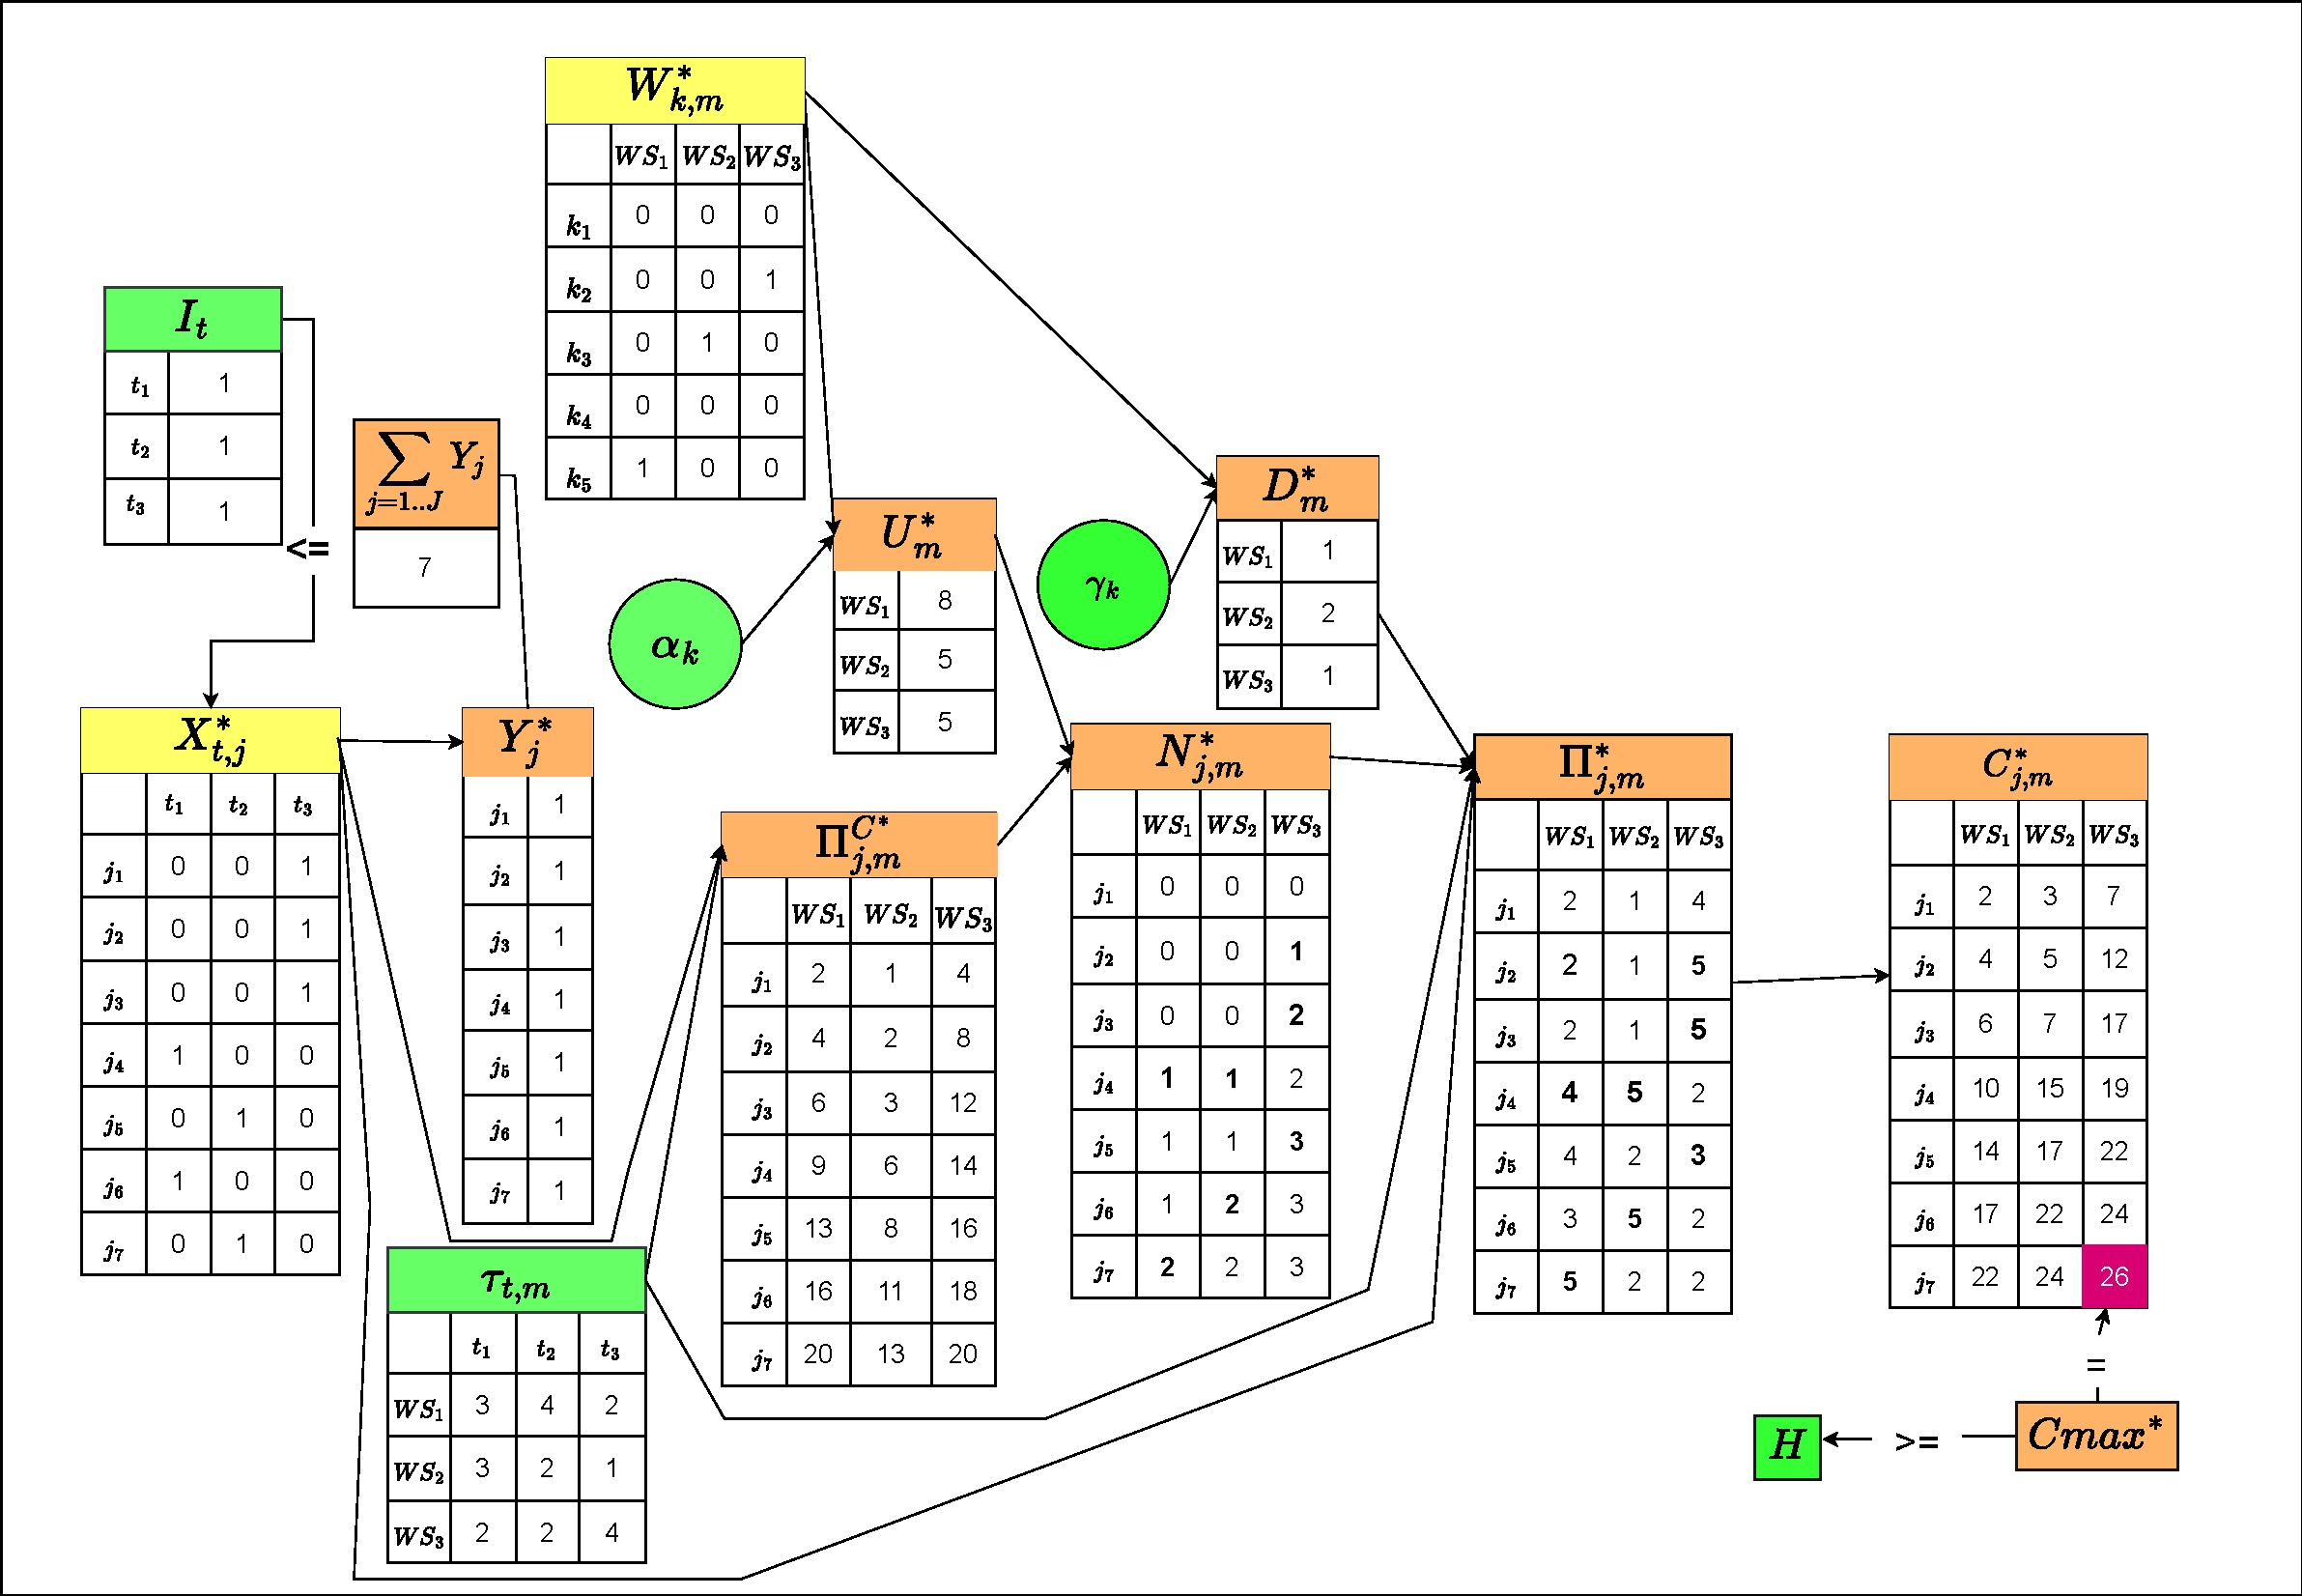
\includegraphics[width=\textwidth]{Example.pdf}}
	\caption{Decision variables and their links with parameters through the illustrative example}
	\label{fig:Ex_p3}
\end{figure}
	
Consider the optimal solution generated by the optimization process. By combining the assignments of the workers ($W^*_{k,m}$) with their respective profiles ($f_{k,p}$), we are able to obtain the ideal assignment of profiles to workstations, represented by $M^*_{p,m}=\sum_{k \in\mathcal{K}} W^*_{k,m} f_{k,p} \ \forall{p\in \mathcal{P},m \in \mathcal{M}} $. This optimal assignment not only maximizes the efficiency of the production system but also ensures that each worker is assigned to a task that best aligns with their particular behavior. To show the efficiency of the model in the case of several products, we set the minimum demand vector $I$. 
To better understand and verify the results, we present the Gantt chart of the optimal solution obtained in Figure~\ref{fig:Ex_p4}. The production horizon is limited to 26 time periods, within which seven jobs are processed. The optimization algorithm has assigned worker k=5, belonging to profile~2, to workstation~1, worker~3, belonging to profile~3, to workstation~2, and worker~2, belonging to profile~1, to workstation~3. Furthermore, the algorithm schedules the jobs by starting with three jobs of type~3 (in blue), followed by one job of type~1 (orange), one job of type~2 (green), one job of type~1 (orange), and finally, the last job of type~2 (green).
	
Different times used for the implementation of the algorithm are illustrated, such as processing time ($\tau_{t,m}$), completion time ($C_{j,m}$), and cumulative processing time ($\Pi^C_{j,m}$). This example demonstrates that the proposed model provides a feasible and \replaced[]{ logical }{ logic } solution that takes into account different human profiles and different workers belonging to different profiles.  
					
\begin{figure}[htbp]
	\centering
	\rotatebox{0}{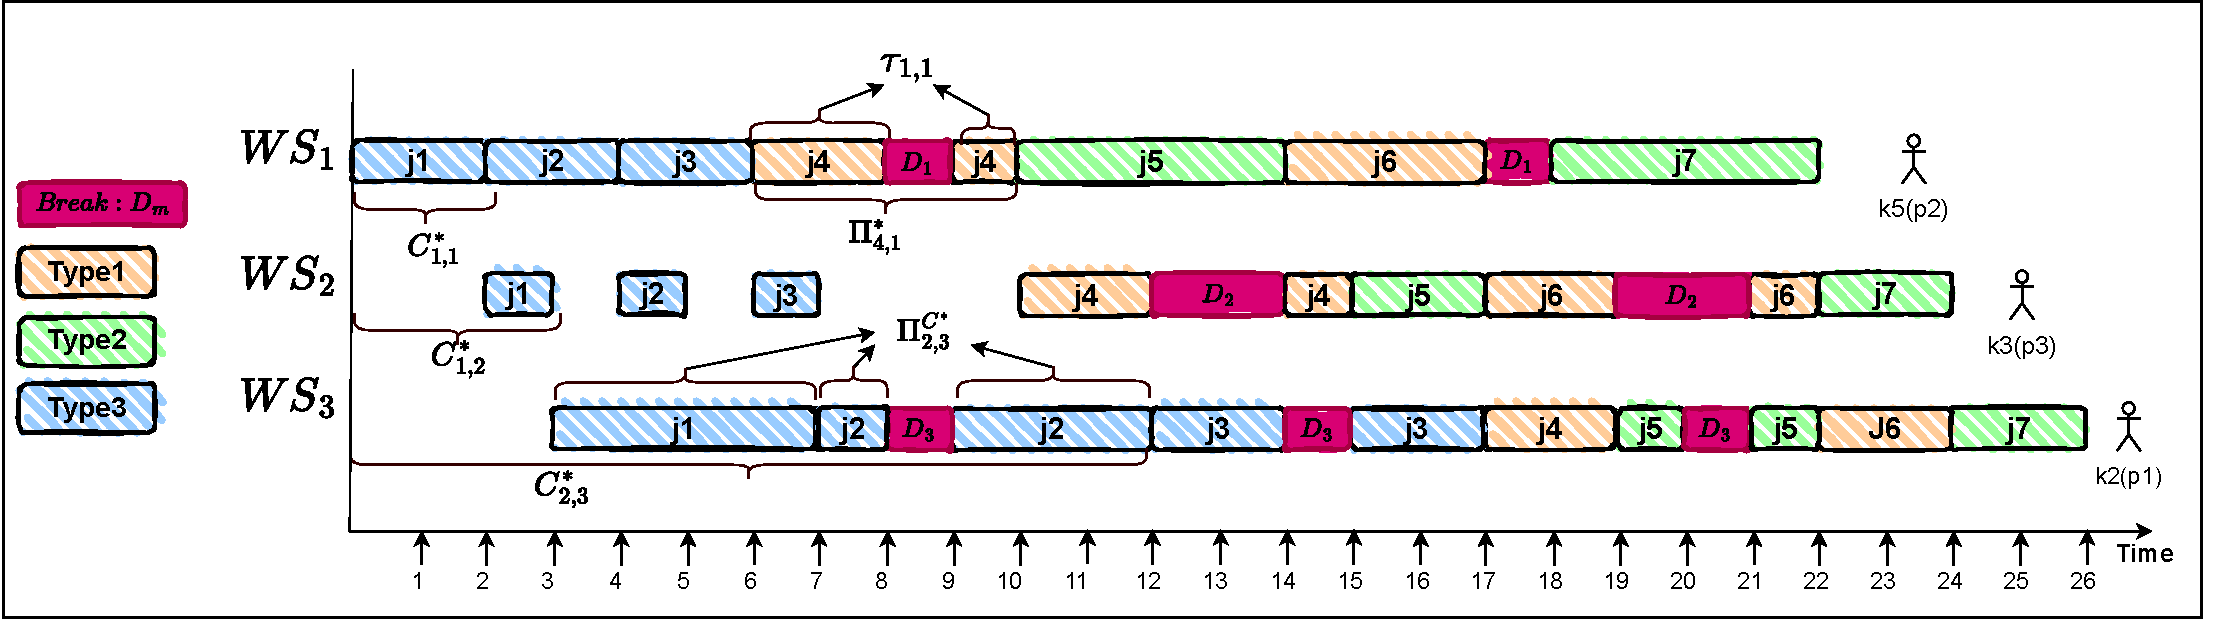
\includegraphics[width=\textwidth]{EX_Gantt.pdf}}
	\caption{Gantt chart of the obtained solution of the illustrative example}
	\label{fig:Ex_p4}
\end{figure}
									
\section{Numerical experiments and discussion}\label{sec:Exp_dis}
\subsection{Simulation results}
We employed the NetLogo 6.2.1 software, equipped with its programming language designed for multi-agent \replaced[comment]{ modeling }{ modelling }systems (MAS), to develop the simulator based on our MAS model (see Figure~\ref{fig:simulator}). Our simulations were based on an example inspired by a case study of the annual preparation of educational robots used in the robotics practical works of a French engineering school. This enables the determination of the number of workstations, the processing time for each one, and the identification of distinct non-productive zones. Although the observation of the use case \replaced[comment=$R1^{11}$]{ does not }{ doesn't } allow for the definition of six profiles, we've created additional profiles to encompass a broad range of profiles, from the robotic profile to the non-punctual profile that spends only 70\% of its time in the productive zone. Given that the use case entails six workstations, we presume that, in the ideal scenario, each worker is exclusively assigned to one workstation. The simulation represented a \replaced[comment]{ dual-resource-constrained }{ dual-resource constrained } flow-shop production system consisting of six workstations in the productive zone and three non-productive zones that represent reasons for workers to temporarily leave their workstation, such as a personnel call, lunch break, or treatment in the infirmary as presented in Figure~\ref{fig:simulator}. Each worker was responsible for performing one or several specific production operations using a set of equipment associated with their workstation. The use of the simulator allows us to show the movement of workers \deleted[]{ that can move }{} between the workstations ($WS_i$) and the non-productive zones. The product \added[]{ is } represented by boxes moving through the production line. Their transformation is represented by a modification of the \replaced[]{ color }{ colour } of the product from black to white.
\begin{figure}[htbp]
	\centering
	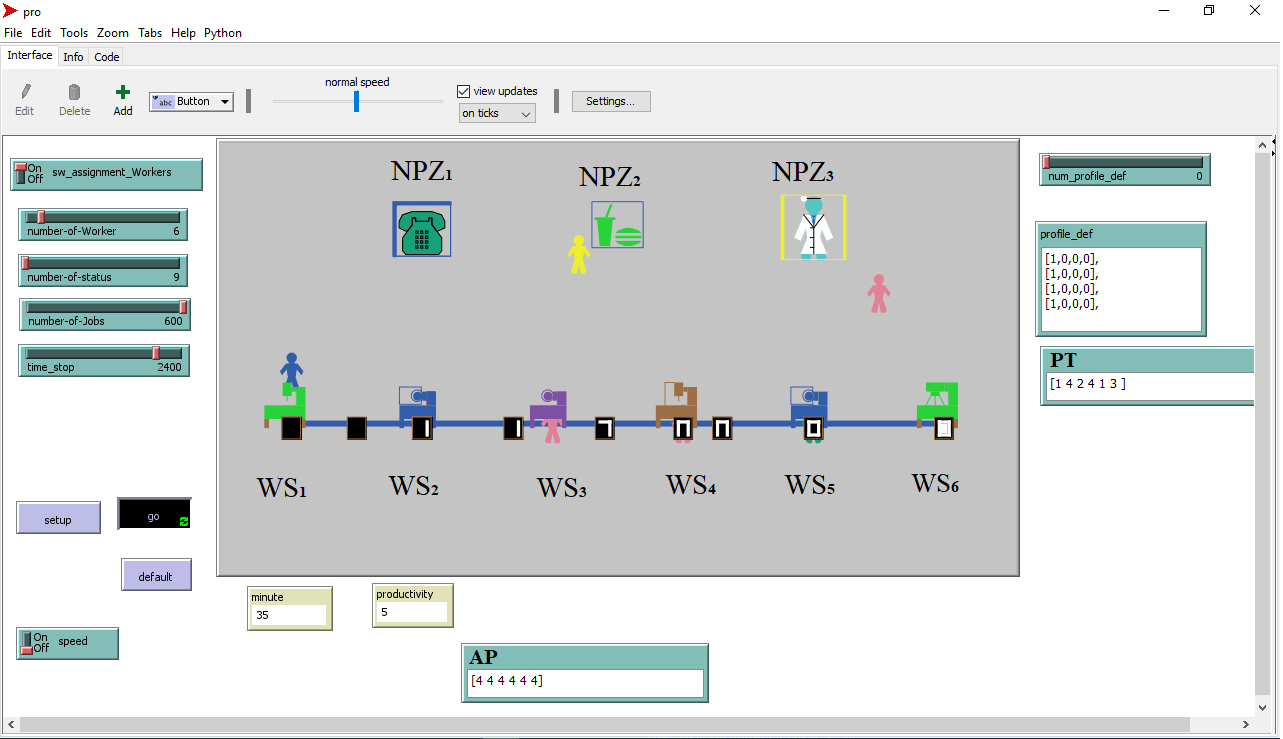
\includegraphics[width=10cm]{simulation.png}
	\caption{Overview of the simulation environment}
	\label{fig:simulator}
\end{figure}
		
To study the impact of different human \replaced[]{behaviors }{ behaviours} on the productivity of dual-resource (human and machine) production systems, we conducted multiple simulations using a Markov chain-based model of human \replaced[comment]{ behavior }{ behaviour } within a multi-agent system (MAS). In each simulation, the workers were assigned specific operations based on their workstation, and their movements between 'productive' and 'non-productive' states were determined by their \replaced[comment]{ behavioral }{  behavioural } profile. Six different profiles of worker \replaced[comment]{ behavior }{ behaviour } were proposed, each represented by a Markov chain with its own transition matrix. The six profile matrices were empirically designed to represent a range between two different extreme situations: i) workers who remain at their workstation throughout the working time and do not move to any NPZ, and ii) workers who tend to have short tenures at the workplace and frequently move between different NPZs. 
To define \added[]{ the } parameters of any model like ours, the majority of existing studies are based on data from case studies, datasets or hypotheses. Although we reviewed some data in the literature, we found that it was not suitable for our study, as some were inapplicable to a production system such as ours (e.g., construction industry), while others did not allow us \deleted[]{to} to generate exploitable profile matrices (e.g., datasets of MTBI personality type test). This is why we adopted an empirical approach to define different behavioral profiles, including, in particular, two extreme cases of profiles in order to enrich our analysis. These matrices were used to differentiate between the various worker profiles. The six generic profiles of worker \replaced[comment]{ behavior }{ behaviour } were represented by the following Markov chain transition matrices:
\counterwithout{table}{section}
\begin{table}[htbp] 
	\centering
	\begin{tabular}{ccc}
		& & \\
		$ P^0 = \left( {\begin{array}{cccc}
		1    & 0    & 0   & 0   \\
		1    & 0    & 0   & 0   \\
		1    & 0    & 0   & 0   \\
		1    & 0    & 0   & 0   \\
		\end{array} } \right)$ 
		&
		$P^1 = \left({\begin{array}{cccc}
		0.95 & 0.05 & 0   & 0   \\
		0.95 & 0.05 & 0   & 0   \\
		1    & 0    & 0   & 0   \\
		1    & 0    & 0   & 0   \\
		\end{array} } \right)$  \\
		& \\
		$P^2 = \left( {\begin{array}{cccc}
		0.9  & 0.1  & 0   & 0   \\
		0.95 & 0.05 & 0   & 0   \\
		1    & 0    & 0   & 0   \\
		1    & 0    & 0   & 0   \\
		\end{array} } \right)$ 
		&
		$P^3 = \left( {\begin{array}{cccc}
		0.7  & 0.3  & 0   & 0   \\
		0.95 & 0.05 & 0   & 0   \\
		1    & 0    & 0   & 0   \\
		1    & 0    & 0   & 0   \\
		\end{array} } \right)$ \\
		& \\
		$P^4 = \left( {\begin{array}{cccc}
		0.7  & 0.3  & 0   & 0   \\
		0.7  & 0.3  & 0   & 0   \\
		1    & 0    & 0   & 0   \\
		1    & 0    & 0   & 0   \\
		\end{array} } \right)$ 
		&
		$P^5 = \left( {\begin{array}{cccc}
		0.8  & 0.2  & 0   & 0   \\
		0.6  & 0.2  & 0.1 & 0.1 \\
		0    & 0.3  & 0.4 & 0.3 \\
		0    & 0.3  & 0.3 & 0.4 
		\end{array} } \right)$			
	\end{tabular}\\
	\label{tab:mytable}
\end{table}

Each Markov chain consists of four states, which are determined by the workers' positions and activities. The workers can either be in a productive zone, where they are working at their assigned workstations (PZ), or a non-productive zone (NPZ). The NPZ is where workers can be found taking a coffee or lunch break, making a personal call or taking a bathroom break, or being in the infirmary for care.
	
The transition probabilities between these states differ depending on the worker profile. The profiles considered in the simulation aim to cover all possible situations, ranging from the “as-" profile ($P^0$), where the worker does not move from the working zone, to the 'undisciplined/disruptive' profile such as profile $P^5$. 
In this simulation example, we make the following assumptions: i) only one type of product is manufactured, ii) each worker is assigned to a single and permanent workstation, iii) product transfer time between workstations is negligible, and iv) there is no setup time or changeover time between production runs.

Other input parameters used in the simulation are as follows:
\begin{itemize}
    \item Simulation time horizon: 1 week of 5 working days, 8 hours per day
    \item Workstations' processing times:\\ $PT=[1,4,2,4,1,3]$ for the workstations $\textit{WS}_1$ to $\textit{WS}_6$, respectively.
    \item Workers' profiles: $P^0$ (Ideal), $P^1$, $P^2$, $P^3$, $P^4$ and $P^5$ 
    \item Scenarios of profiles assignment: we simulated 36 scenarios, representing different combinations of workers' profiles assigned to workstations.
        \begin{itemize}
            \item  \textit{Global scenarios (6)}:
                \begin{itemize}
                    \item 	 \hspace*{0.5cm} G0: $AP=[0,0,0,0,0,0]$ (Perfect)
                    \item    \hspace*{0.5cm} Gk: $AP=[k,k,k,k,k,k]$, $k=1,2,..,5$ 
                \end{itemize}
            \item  \textit{Mixed scenarios (30)}: 
                \begin{itemize}
                    \item 	  \hspace*{0.5cm} Mk1: $AP=[k,0,0,0,0,0]$, $k=1,2,..,5$
                    \item     \hspace*{0.5cm} Mk2: $AP=[0,k,0,0,0,0]$, $k=1,2,..,5$
                    \item    \hspace*{0.5cm} Mk3: $AP=[0,0,k,0,0,0]$, $k=1,2,..,5$
                    \item    \hspace*{0.5cm} Mk4: $AP=[0,0,0,k,0,0]$, $k=1,2,..,5$
                    \item    \hspace*{0.5cm} Mk5: $AP=[0,0,0,0,k,0]$, $k=1,2,..,5$
                    \item    \hspace*{0.5cm} Mk6: $AP=[0,0,0,0,0,k]$, $k=1,2,..,5$
                \end{itemize}
        \end{itemize}
    \item Gk: the value of the Global scenarios
    \item {\it{\%gap}}:  The percentage gap of the productivity of a given scenario ($\pi(s)$) compared to a reference scenario ($\pi(s^0)$),  $\textit{\%gap}=\frac{ \pi(s) - \pi(s^0)}{\pi(s^0)}$.
\end{itemize}

\setcounter{table}{0}
\begin{table}[htbp]
    \begin{center}
        \begin{longtable}{|cc|cccccc|ccc|}
	    \hline
	    \multicolumn{2}{|c|}{} & \multicolumn{6}{c|}{Operator profiles assignment}& \multicolumn{2}{c}{Productivity (u)}&\\
            \# & ID  & $\textit{WS}_1$ & $\textit{WS}_2$ & $\textit{WS}_3$ & $\textit{WS}_4$ & $\textit{WS}_5$ & $\textit{WS}_6$ & 
			& Gk   & \it{\%gap} \\ 
			\hline
			1  & G0  & 0 & 0 & 0 & 0 & 0 & 0 & 597 & -   & -    \\
			2  & G1  & 1 & 1 & 1 & 1 & 1 & 1 & 564 & -   & -    \\
			3  & G2  & 2 & 2 & 2 & 2 & 2 & 2 & 564 & -   & -    \\
			4  & G3  & 3 & 3 & 3 & 3 & 3 & 3 & 533 & -   & -    \\
			5  & G4  & 4 & 4 & 4 & 4 & 4 & 4 & 533 & -   & -    \\
			6  & G5  & 5 & 5 & 5 & 5 & 5 & 5 & 563 & -   & -    \\
			\hline
			7  & M11 & 1 & 0 & 0 & 0 & 0 & 0 & 597 & 564 & 5.9  \\
			8  & M12 & 0 & 1 & 0 & 0 & 0 & 0 & 567 & 564 & 0.5  \\
			9  & M13 & 0 & 0 & 1 & 0 & 0 & 0 & 597 & 564 & 5.9  \\
			10 & M14 & 0 & 0 & 0 & 1 & 0 & 0 & 567 & 564 & 0.5  \\
			11 & M15 & 0 & 0 & 0 & 0 & 1 & 0 & 597 & 564 & 5.9  \\
			12 & M16 & 0 & 0 & 0 & 0 & 0 & 1 & 597 & 564 & 5.9  \\
			\hline
			13 & M21 & 2 & 0 & 0 & 0 & 0 & 0 & 597 & 564 & 5.9  \\
			14 & M22 & 0 & 2 & 0 & 0 & 0 & 0 & 567 & 564 & 0.5  \\
			15 & M23 & 0 & 0 & 2 & 0 & 0 & 0 & 597 & 564 & 5.9  \\
			16 & M24 & 0 & 0 & 0 & 2 & 0 & 0 & 567 & 564 & 0.5  \\
			17 & M25 & 0 & 0 & 0 & 0 & 2 & 0 & 597 & 564 & 5.9  \\
			18 & M26 & 0 & 0 & 0 & 0 & 0 & 2 & 597 & 564 & 5.9  \\
			\hline
			19 & M31 & 3 & 0 & 0 & 0 & 0 & 0 & 597 & 533 & 12.0 \\
			20 & M32 & 0 & 3 & 0 & 0 & 0 & 0 & 535 & 533 & 0.4  \\
			21 & M33 & 0 & 0 & 3 & 0 & 0 & 0 & 597 & 533 & 12.0 \\
			22 & M34 & 0 & 0 & 0 & 3 & 0 & 0 & 537 & 533 & 0.8  \\
			23 & M35 & 0 & 0 & 0 & 0 & 3 & 0 & 597 & 533 & 12.0 \\
			24 & M36 & 0 & 0 & 0 & 0 & 0 & 3 & 597 & 533 & 12.0 \\
			\hline
			25 & M41 & 4 & 0 & 0 & 0 & 0 & 0 & 597 & 533 & 12.0 \\
			26 & M42 & 0 & 4 & 0 & 0 & 0 & 0 & 537 & 533 & 0.8  \\
			27 & M43 & 0 & 0 & 4 & 0 & 0 & 0 & 597 & 533 & 12.0 \\
			28 & M44 & 0 & 0 & 0 & 4 & 0 & 0 & 538 & 533 & 0.9  \\
			29 & M45 & 0 & 0 & 0 & 0 & 4 & 0 & 597 & 533 & 12.0 \\
			30 & M46 & 0 & 0 & 0 & 0 & 0 & 4 & 597 & 533 & 12.0 \\
			\hline
			31 & M51 & 5 & 0 & 0 & 0 & 0 & 0 & 597 & 563 & 6.0  \\
			32 & M52 & 0 & 5 & 0 & 0 & 0 & 0 & 566 & 563 & 0.5  \\
			33 & M53 & 0 & 0 & 5 & 0 & 0 & 0 & 597 & 563 & 6.0  \\
			34 & M54 & 0 & 0 & 0 & 5 & 0 & 0 & 568 & 563 & 0.9  \\
			35 & M55 & 0 & 0 & 0 & 0 & 5 & 0 & 597 & 563 & 6.0  \\
			36 & M56 & 0 & 0 & 0 & 0 & 0 & 5 & 597 & 563 & 6.0  \\
			\hline
		\end{longtable}
		\caption{Results of all tested scenarios (Simulation)}
		\label{tab:t0}
	\end{center}
\end{table}
	
Table~\ref{tab:t0} presents the simulation results, showing the level of productivity achieved by each scenario. \added[comment=$R1^{13}$]{Each scenario in Table~\ref{tab:t0} is defined by a number and an ID. The columns ``operator profile assignment" display the ID of the profile assigned to each Workstation. In the ``Productivity" columns, is shown the simulated productivity of the scenario, followed by the simulated productivity of the global scenario of this profile, and finally, the gap between these two values. For example, in scenario 31, which has the ID $M51$, the worker of profile 5 is assigned to the workstation $WS_1$ and profile 0 is assigned to all the other workstations. The productivity of this scenario is 597 produced units. Knowing that the number of units produced with profile 5 in the global scenario is 563  (result of the scenario G5), the productivity gap is $6 \%$.}


Out of 35 scenarios, 20 performed equally well as the perfect scenario where all workers have the ideal profile. This finding suggests that the impact of each profile on productivity can vary depending on the workstation to which it is assigned. Further examination of the results reveals that the productivity level decreases significantly when profiles \#3 or \#4 are assigned to bottleneck workstations such as $\textit{WS}_2$ or $\textit{WS}_4$. Therefore, it is evident that the allocation of workers to specific workstations affects productivity, and careful consideration of the profiles of the workers is necessary to optimize overall productivity.
	
Based on the results, we \replaced[]{aim}{will attempt} to discuss the effect of operator placement \replaced[]{along}{on} the production line and how \replaced[]{to take advantage of performance disparities, thereby optimizing operator assignment for increased productivity.}{one can benefit from the performance difference to place these operators in a favorable position}.
Figure~\ref{fig:glo_mix} displays the percentage decrease in productivity, compared to the perfect profile, 
for each profile in both mixed scenarios (on average) and global scenarios. For example, if profile \#2 is assigned to all workstations (global scenario), there is a reduction \added[]{ of } 6\% in productivity compared to the perfect profile (green bar). However, in the mixed scenario, this reduction drops to an average of 2\% (red bar).

\begin{figure}[htbp]
    \centering								
    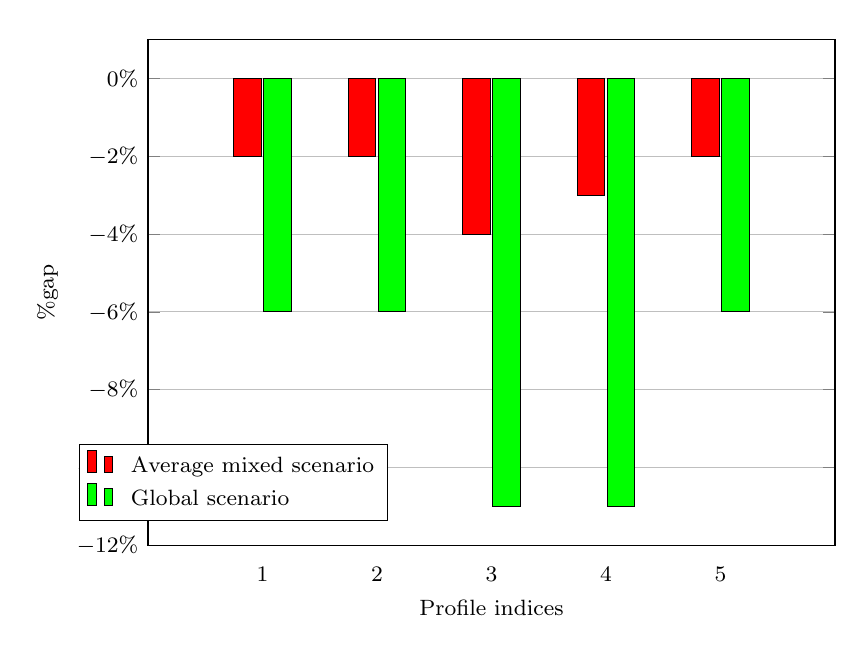
\begin{tikzpicture}[font=\footnotesize,baseline]
	\begin{axis}[width  = 0.85*\textwidth,
                    height = 8cm,
				major x tick style = transparent,
				ybar=2*\pgflinewidth,
				bar width=10pt,
				ymajorgrids = true,
				ymin=-12,
				ymax=1,
				yticklabel={\pgfmathparse{\tick}\pgfmathprintnumber{\pgfmathresult}\%},
				xtick = data,
                    xlabel ={Profile indices},
                    ylabel = {\%gap},
				scaled y ticks = false,
				enlarge x limits=0.25,
				legend cell align=left,
				legend entries={Average mixed scenario, Global scenario},
				legend style={ 
                        at={(0.35,0.2)},
					anchor=north east,
					column sep=1ex
				}
			]								
            \addplot[color=black, fill=red,mark=none] coordinates {(1,-2)(2,-2)(3,-4)(4,-3)(5,-2)};
		\addplot[color=black,fill=green,mark=none] coordinates {(1,-6)(2,-6)(3,-11)(4,-11)(5,-6)};
	\end{axis}
    \end{tikzpicture}
    \caption{Effect of profile assignment strategies on productivity}
    \label{fig:glo_mix}
\end{figure}

The \replaced[]{ profiles }{ profile } with the highest average slowdown in productivity are \#3 and \#4, which results in \replaced[]{ an }{ a }11\% reduction. This is because the probability of staying at a workstation is only $0.7$ in the corresponding Markov chain.

Based on the results above, we can define \deleted[]{ for each profile } a ranking of workstation assignments regarding the throughput performance \added[]{ for each profile (see Table~\ref{tab:t2}}. The ideal worker profile is ranked first for all workstations, which means that we obtain the maximum throughput when it is placed in any workstation. The other \replaced[]{worker's profiles reduce  }{ worker profile are reducing }    the throughput when \deleted[]{they are} placed on the bottleneck stations (\#2 and \#4). For \replaced[]{ profiles }{ profile } $P_1$ and $P_2$, the assignment of the worker to $\textit{WS}_1$, $\textit{WS}_3$, $\textit{WS}_5$, or $\textit{WS}_6$ \replaced[]{ gives }{ is giving }{}the maximum throughput of 597 (Rank1), followed by  $\textit{WS}_2$ and  $\textit{WS}_4$ with a throughput of 567 (Rank2).  Similarly, Profiles $P_3$, $P_4$, and $P_5$ are best ranked with workstations $\textit{WS}_1$, $\textit{WS}_3$, $\textit{WS}_5$, or $\textit{WS}_6$ \deleted[]{ that }{}have the lowest processing time, and \replaced[]{ obtain }{ obtaining }{} a rank 2 when assigned to $\textit{WS}_4$ with a throughput of 538, it also obtains the rank 3 when assigned to the $\textit{WS}_2$ with a throughput of 537.

\begin{table}[h!]
	\begin{center}
		\caption{Ranked best workstation assignments for each worker profile}\label{tab:t2}
		\begin{tabular}{cccc}
					Profile & Rank1 & Rank2 & Rank3  \\\hline
					0       & 1,2,3,4,5,6 & -       & -   \\ 
					1       & 1,3,5,6    & 2,4      & -   \\ 
					2       & 1,3,5,6    & 2,4      & -   \\ 
					3       & 1,3,5,6   & 4         & 2   \\ 
					4       & 1,3,5,6   & 4       & 2   \\
					5       & 1,3,5,6    & 4        & 2    \\ \hline
					\\
				\end{tabular}
	\end{center}
\end{table}


Although the chosen scenarios are very restrictive, these results demonstrate how human \replaced[comment]{ behavior }{ behaviour } can negatively impact productivity and highlight the importance of an optimized allocation of different worker profiles to workstations. To address this issue, the following section proposes an effective optimization method for selecting the most suitable allocation of a group of workers with diverse \replaced[comment]{ behavioral }{  behavioural } profiles to a given number of workstations.

\subsection{\replaced[]{ Optimization }{ Optimisation }{} results}
The mathematical model presented in the previous section has been implemented using the  Gurobi optimization solver library within Julia programming language.\added[]{ The different experiments have been run on a PC with Intel(R) Core(TM) i9-14900HX 2.20 GHz CPU 2.40 GHz processor and 32.0 GB RAM.} 
We conducted experiments using the same instance as the experiments using the simulation method described in the previous section, which included six workstations and six distinct \replaced[]{ behavioral }{ behavioural }{} profiles of workers. Furthermore, we considered three different types of products in our analysis $\{t1, t2, t3\}$.
Other input parameters used in the optimization process are as follows: 
\begin{itemize}
    \item The production mix: $(I_1, I_2, I_3)$
    \item  The processing times $\tau_{t,m}$ of each product type on each workstation are given as follows: 
        \begin{itemize}
            \item $t1$: $\textit{WS}1(1)$, $\textit{WS}2(4)$, $\textit{WS}3(2)$, $\textit{WS}4(4)$, $\textit{WS}5(1)$, $\textit{WS}6(3)$ with a nominal cycle time of 4
            \item $t2$: $\textit{WS}1(2)$, $\textit{WS}2(1)$, $\textit{WS}3(2)$, $\textit{WS}4(1)$, $\textit{WS}5(4)$, $\textit{WS}6(3)$ with a nominal cycle time of 4
            \item $t3$: $\textit{WS}1(1)$, $\textit{WS}2(3)$, $\textit{WS}3(3)$, $\textit{WS}4(3)$, $\textit{WS}5(3)$, $\textit{WS}6(3)$ with a nominal cycle time of 3
        \end{itemize}
    \item $H$   time horizon of production  2400 minute   
    \item$\lambda^1_p$ average duration of the working time period of a worker with profile $p$. The values of this parameter for profiles $p_0$, $p_1$, $p_2$, $p_3$, $p_4$, and $p_5$  are respectively 2400, 94, 85,  43.5, 38 and 80	
    \item $\lambda^0_p$ average duration of the absence time period of a worker with profile $p$. The values of this parameter for profiles $p_0$, $p_1$, $p_2$, $p_3$, $p_4$, and $p_5$  are respectively 1, 5, 4.9, 4.7, 4.6 and 4.8.      
\end{itemize}

To capture the potential variability in worker profiles and production mix, we defined 75 unique scenarios, each with varying numbers of workers belonging to each profile and production mix. These scenarios were then \replaced[]{ organized }{ organised }{} into nine distinct groups, \replaced[]{ labeled }{ labelled }{} “GA" to “GI", as follows:
\begin{itemize}
    \item In the Group A scenarios, six workers with the same profile are assigned to test the overall impact of this profile on +productivity and to classify the profiles. 
    \item In the scenarios of Group B, 5 workers with profile 0 (perfect profile) and 1 worker with a different profile are assigned to deduce the partial impact of each profile on each \replaced[comment]{ workstation}{ machine }.
    \item In the scenarios of Groups C, D, E, and F, the same strategy as in Scenario B is adopted, but with a gradual decrease in the number of workers with profile 0. This will allow testing the partial effect of each profile \deleted[]{,}{} while the other \replaced[comment]{ workstations }{ machines } are perfect. 
    \item The scenario of Group G is a scenario in which the profiles were randomly selected to study the impact of a combination of profiles on productivity.
    \item  In all scenarios (A to G), only the production of a type 1 product is allowed in order to test only the effect of the worker allocation on the productivity of the system.
    \item In scenarios of Group H, we allow the production of several types of products to test the effect of profile allocation and scheduling of jobs on the productivity of the system.  
\end{itemize}
					
In order to assess the efficiency of the optimal solution, the latter is compared to the “worst assignment" solution for each scenario. The worst assignment of workers to jobs is achieved by iteratively assigning the most undisciplined worker (highest ratio $\lambda^0_p/(\lambda^0_p+\lambda^1_p)$) to the most important production \replaced[comment]{ workstation }{ machine } (bottleneck) and vice versa.
					
Each scenario runs on a time horizon of one week of five working days, eight hours per day, that is, $H=2400$ hours. The result of each tested scenario is \replaced[]{ characterized }{ characterised }{} by:
	
\begin{tabular}{p{.13\textwidth} p{.8\textwidth}}
	\it{GR}                                  & ID of the group of scenarios, GA to GH                                 \\
	\it{ID}                                  & ID  of scenario, which is its number that ranges from 1 to 62          \\
	$(n_0,..,n_5)$                           & Number of workers available in each profile $p\in \{0, 1, 2, 3, 4,5\}$ \\       
	$(I_1,..,I_3)$                           & Production mix, where:                                                 \\
	                                         & $I_t= \left\{                                                          
	\begin{array}{ll}
	0                                        & \text{if the type $t$ product should not be produced}                  \\
	q_t^{min}                                & \text{if at least $q_t^{min}$ products of type $t$ must be produced}   \\
	\end{array} \right.$\\
	$(a^*_1,..,a^*_6)$                       & Optimal assignment of profiles to workstations.                        \\
	\it{obj}$^*$                             & Productivity (throughput) of the optimal solution.                     \\
	$(q^*_1$,..,$q^*_3)$                     & Optimal quantities for each type of product.                           \\
	$(a^{\textsc{w}}_1,..,a^{\textsc{w}}_6)$ & Worst assignment of profiles to workstations.                          \\
	\it{obj}$^{\textsc{w}}$                  & Productivity of the worst solution.                                    \\
	\it{\%gap}                               & Percentage gap of the worst solution compared to the optimal one:      \\
	                                         & $\%gap=\displaystyle\frac{obj^* - obj^{\textsc{w}}}{obj^*}$. \\
        \added[]{\it{cpu [min]}}                               & \added[]{Computation time in minutes.}\\
\end{tabular}\\

The results of the defined scenarios are presented in Table~\ref{tab:tr_ga}, Table~\ref{tab:tr_gb}, Table~\ref{tab:tr_gcdef}, and Table \ref{tab:tr4}. 	
								
\setlength{\tabcolsep}{3pt}
\setcounter{table}{2}
\begin{longtable}{|c|c|c|c|c|c|c|c|c|r|r|}
    \hline
    & & \multicolumn{2}{c|}{Inputs} & \multicolumn{3}{c|}{Optimal assignment} & &  \\
    & \multicolumn{1}{c|}{ } & \multicolumn{1}{c|}{Profiles} & \multicolumn{1}{c|}{Mixprod}& \multicolumn{1}{c}{}  & \multicolumn{2}{c|}{} &\multicolumn{1}{c|}{}&\\
    \it{GR} & \it{ID} & \multicolumn{1}{c|}{$(n_0,..,n_5)$} & \multicolumn{1}{c|}{$(I_1,..,I_3)$} & {$(a^*_1,..,a^*_6)$} & \it{obj}$^*$ & $(q^*_1$,...,$q^*_3)$  & \it{\%gap} & \it{ cpu [min]}  \\
    \hline
	        & 1       & 6,0,0,0,0,0                         & 1,0,0                               & 0,0,0,0,0,0          & 597          & 597,0,0                                    & 0.0 (Ref.)     & 9.2     \\
	        & 2       & 0,6,0,0,0,0                         & 1,0,0                               & 1,1,1,1,1,1          & 567          & 567,0,0                                    & 5.0    & 10.5     \\
	        & 3       & 0,0,6,0,0,0                         & 1,0,0                               & 2,2,2,2,2,2          & 564          & 564,0,0                                    & 5.5    & 10.4  \\
	{GA}%\label{SEN:GA} 
	        & 4       & 0,0,0,6,0,0                         & 1,0,0                               & 3,3,3,3,3,3          & 536          & 536,0,0                                    & 10.2    & 10.4 \\
	        & 5       & 0,0,0,0,6,0                         & 1,0,0                               & 4,4,4,4,4,4          & 528          & 528,0,0                                    & 11.5     & 10.3\\
	        & 6       & 0,0,0,0,0,6                         & 1,0,0                               & 5,5,5,5,5,5          & 562          & 562,0,0                                    & 5.8     & 10.4  \\
	\hline
	\caption{Results of the scenarios of Group A}
	\label{tab:tr_ga}
\end{longtable}


From Table~\ref{tab:t0} and Table~\ref{tab:tr_ga}, we conducted a comparative analysis of the results obtained through simulation and those obtained through \replaced[]{ optimization }{ optimisation }{}. The results show that the two methods are equivalent and that the perfect profile ("Profile 0") allows for the maximum value of the objective function to be achieved. Moreover, the tested profiles can be ranked in terms of their efficiency, from the most effective to the least effective, as follows: 0, 1, 2, 5, 3, and 4. 

\begin{figure}[htbp]
	\centering	    
	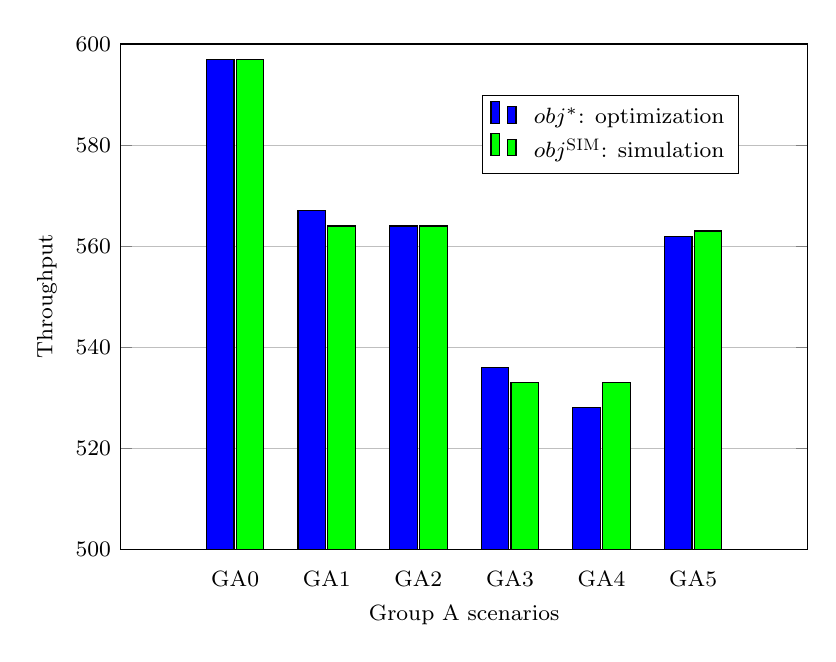
\begin{tikzpicture}[font=\footnotesize,baseline]
		\begin{axis}[
				width  = 0.85*\textwidth,
				height = 8cm,
				major x tick style = transparent,
				ybar=2*\pgflinewidth,
				bar width=10pt,
				ymajorgrids = true,
				ymin=500,
				ymax=600,
                xlabel = {Group A scenarios},
				ylabel = {Throughput},
				xticklabel={GA\pgfmathprintnumber\tick},
				xtick = data,
				scaled y ticks = false,
				enlarge x limits=0.25,
				legend cell align=left,
				legend entries={$obj^*$: optimization, $obj^{\textsc{SIM}}$: simulation},
				% legend to name=named,
				legend style={
					at={(0.9,0.9)},
					anchor=north east,
					column sep=1ex
				}
			]
			\addplot[color=black, fill=blue,mark=none] coordinates {(0,597)(1,567)(2,564)(3,536)(4,528)(5,562)};
			\addplot[color=black,fill=green,mark=none] coordinates {(0,597)(1,564)(2,564)(3,533)(4,533)(5,563)};
		\end{axis}
	\end{tikzpicture}
	\caption{Comparison of profiles across global assignment scenarios results}

	\label{fig:88}
\end{figure}
			
					
\begin{longtable}{|c|c|c|c|c|c|c|c|c|r|r|}
	\hline
	& & \multicolumn{2}{c|}{Inputs} & \multicolumn{3}{c|}{Optimal assignment} & \multicolumn{2}{c|}{Worst assignment }& \multicolumn{2}{c|}{}\\
	&  & Profiles & Mixprod & \multicolumn{3}{c|}{} & \multicolumn{2}{c|}{} & \multicolumn{2}{c|}{}\\
    \it{GR} & \it{ID} & \multicolumn{1}{c|}{$(n_0,..,n_5)$} & \multicolumn{1}{c|}{$(I_1,..,I_3)$} & {$(a^*_1,..,a^*_6)$} & \it{obj}$^*$ & $(q^*_1$,...,$q^*_3)$ & {$(a^{\textsc{w}}_1,..,a^{\textsc{w}}_6)$} & \it{obj}$^{\textsc{w}}$ & \it{\%gap}   & \it{ cpu [min]} \\	
	\hline
	        & 7       & 5,1,0,0,0,0                         & 1,0,0                               & 1,0,0,0,0,0          & 597          & 597,0,0               & 0,1,0,0,0,0                                & 567                     & 5.0      & 10.3  \\
	        & 8       & 5,0,1,0,0,0                         & 1,0,0                               & 2,0,0,0,0,0          & 597          & 597,0,0               & 0,2,0,0,0,0                                & 564                     & 5.5        & 10.3   \\
	GB      & 9       & 5,0,0,1,0,0                         & 1,0,0                               & 0,0,0,0,3,0          & 597          & 597,0,0               & 0,3,0,0,0,0                                & 536                     & 10.2        & 10.2  \\
	        & 10      & 5,0,0,0,1,0                         & 1,0,0                               & 0,0,0,0,4,0          & 597          & 597,0,0               & 0,4,0,0,0,0                                & 528                     & 11.6       & 8.8   \\
	        & 11      & 5,0,0,0,0,1                         & 1,0,0                               & 0,0,0,0,5,0          & 597          & 597,0,0               & 0,5,0,0,0,0                                & 562                     & 5.9        & 8.7   \\
	\hline
	\caption{Results of mixed scenarios  Group B} 													
	\label{tab:tr_gb}
\end{longtable}
										
Table~\ref{tab:tr_gb} presents the results of the scenarios considered in Group B (GB), which are comparable to the mixed scenario in the simulation section (in Table~\ref{tab:t0} -id $\in \{7..12\}$- from M11 to M16). The optimization process provides the optimal assignments of workers with non-perfect profiles, which ensures efficient use of resources and high-quality results.
			
All proposed solutions achieve optimal results when the perfect profile is assigned to the bottleneck \replaced[comment]{ workstations }{ machines } (\replaced[comment]{ workstation }{ machine } 2 and \replaced[comment]{ workstation }{ machine } 4). The worst assignment occurs when the non-perfect profile is assigned to the first bottleneck \replaced[comment]{ workstation }{ machine } (\replaced[comment]{ workstation }{ machine } 2). Similar results can be obtained by assigning the non-perfect profile to the second bottleneck \replaced[comment]{ workstation }{ machine } (Machine 4){\color{red}}. This confirms the classification obtained from the experimentation in group A (see Table~\ref{tab:tr_ga}).
			
\begin{figure}[H]
    \centering
    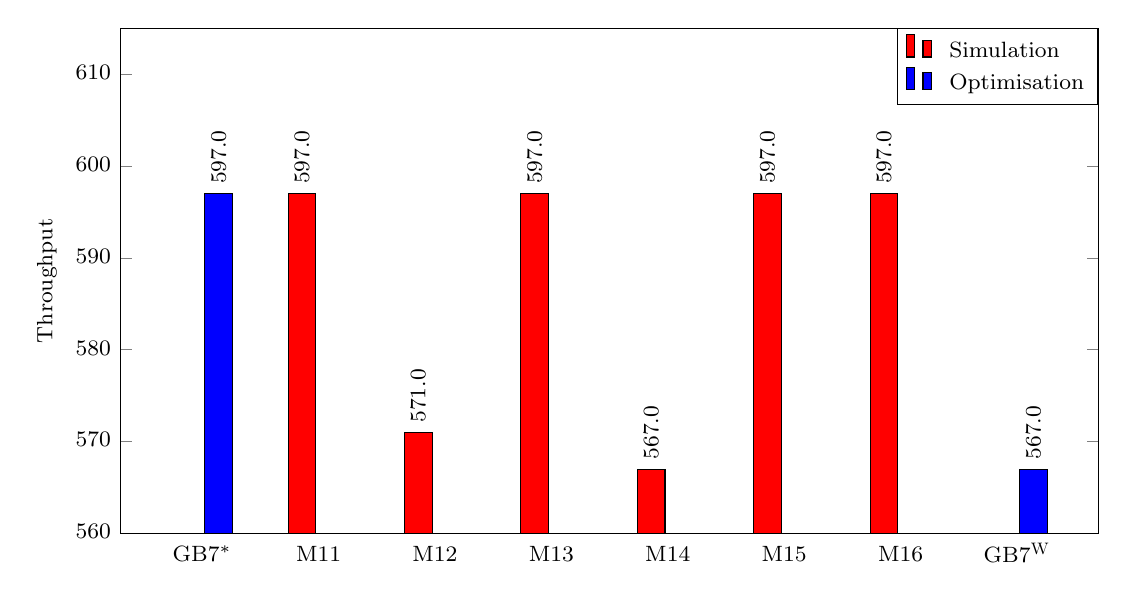
\begin{tikzpicture}[font=\footnotesize,baseline]
        \begin{axis}[
            ybar,
            width=14cm,
            height=8cm,
            ymin=560,
            ymax=615,
            ylabel={Throughput},
            xtick=data,
            xticklabels={GB7$^{*}$,	M11, M12, M13, M14,	M15, M16, GB7$^{\textsc{W}}$},
            typeset ticklabels with strut,
            major tick length=0pt,
            major y tick style={/pgfplots/major tick length=1.5mm},
            nodes near coords always on top/.style={scatter/position=absolute, positive value/.style={
				at={(axis cs:\pgfkeysvalueof{/data point/x},\pgfkeysvalueof{/data point/y})},},
				negative value/.style={at={(axis cs:\pgfkeysvalueof{/data point/x},0)},},
			every node near coord/.append style={
                    check values/.code={%
					\begingroup
					   \pgfkeys{/pgf/fpu}%
					   \pgfmathparse{\pgfplotspointmeta<0}%
					   \global\let\result=\pgfmathresult
					   \endgroup
					   \pgfmathfloatcreate{1}{1.0}{0}%
					   \let\ONE=\pgfmathresult
					   \ifx\result\ONE
					       \pgfkeysalso{/pgfplots/negative value}%
					   \else
						\pgfkeysalso{/pgfplots/positive value}%
					   \fi},
                    check values,
                    anchor=west,
                    rotate=90,
                },
		},
		nodes near coords={\pgfmathprintnumber[fixed zerofill,precision=1]{\pgfplotspointmeta}},
		nodes near coords always on top,
            legend cell align=left,
		legend entries={Simulation, Optimisation},
		legend style={at={(1,1)},
					   anchor=north east,
					   column sep=1ex
		}
        ]			
          \addplot [draw=black,fill=red] coordinates {(0,0)  (1,597) (2,571)  (3,597)  (4,567) (5,597) (6,597) (7,0)};  
	   \addplot [draw=black,fill=blue] coordinates {(0,597) (7,567)};  
        \end{axis}
    \end{tikzpicture}
    \caption{ Variation in throughput among simulated mixed scenarios compared to the throughput achieved with optimal and worst assignments (example for M11 to M16 and GB7) }
   % \caption{Scenario Simulations Mixed k=1 VS Scenario optimization id =7}
    \label{fig:mk1}
\end{figure}
	
To compare optimization results with simulation (Figure~\ref{fig:mk1}) \deleted[]{ones}{} for mixed scenarios, we analyzed, for example, scenario 7 in Table~\ref{tab:tr_gb} to simulations (M11 to M16) (c.f. Table~\ref{tab:t0}) with $k=1$. Simulation results ranged between \added[]{the} worst and best optimization solutions, confirming the reliability of optimization across all scenarios.
	
\begin{longtable}{|c|c|c|c|c|c|c|c|c|c|c|}
	\hline
	& & \multicolumn{2}{c|}{Inputs} & \multicolumn{3}{c|}{Optimal assignment} & \multicolumn{2}{c|}{Worst assignment }& \multicolumn{2}{c|}{}\\
	&  & Profiles & Mixprod & \multicolumn{3}{c|}{} & \multicolumn{2}{c|}{} & \multicolumn{2}{c|}{}\\
    \it{GR} & \it{ID} & \multicolumn{1}{c|}{$(n_0,..,n_5)$} & \multicolumn{1}{c|}{$(I_1,..,I_3)$} & {$(a^*_1,..,a^*_6)$} & \it{obj}$^*$ & $(q^*_1$,...,$q^*_3)$ & {$(a^{\textsc{w}}_1,..,a^{\textsc{w}}_6)$} & \it{obj}$^{\textsc{w}}$ & \it{\%gap}   & \it{ cpu [min]} \\				
	\hline
	        & 12      & 4,2,0,0,0,0                         & 1,0,0                                & 1,0,0,0,1,0          & 597          & 597,0,0               & 0,1,0,1,0,0                                & 567                     & 5.0    &  12.7   \\
	        & 13      & 4,0,2,0,0,0                         & 1,0,0                                & 2,0,0,0,2,0          & 597          & 597,0,0               & 0,2,0,2,0,0                                & 564                     & 5.5   &  16.1     \\
	GC      & 14      & 4,0,0,2,0,0                         & 1,0,0                                & 3,0,0,0,3,0          & 597          & 597,0,0               & 0,3,0,3,0,0                                & 536                     & 10.2     &  16.1   \\
	        & 15      & 4,0,0,0,2,0                         & 1,0,0                                & 4,0,0,0,4,0          & 597          & 597,0,0               & 0,4,0,4,0,0                                & 528                     & 11.5   &  16.2     \\
	        & 16      & 4,0,0,0,0,2                         & 1,0,0                                & 5,0,0,0,0,5          & 597          & 597,0,0               & 0,5,0,5,0,0                                & 562                     & 5.8     &  16.1    \\
	\hline
	        & 17      & 3,3,0,0,0,0                         & 1,0,0                                & 1,0,0,0,1,1          & 597          & 597,0,0               & 0,1,1,1,0,0                                & 567                     & 5.0    &  16.2     \\
	        & 18      & 3,0,3,0,0,0                         & 1,0,0                                & 2,0,0,0,2,2          & 597          & 597,0,0               & 0,2,2,2,0,0                                & 564                     & 5.5   &  12.8     \\
	GD      & 19      & 3,0,0,3,0,0                         & 1,0,0                                & 3,0,0,0,3,3          & 597          & 597,0,0               & 0,3,3,3,0,0                                & 536                     & 10.2   &  12.7    \\
	        & 20      & 3,0,0,0,3,0                         & 1,0,0                                & 4,0,4,0,4,0          & 597          & 597,0,0               & 0,4,4,4,0,0                                & 528                     & 11.5   &  10.9    \\
	        & 21      & 3,0,0,0,0,3                         & 1,0,0                                & 5,0,0,0,5,5          & 597          & 597,0,0               & 0,5,5,5,0,0                                & 562                     & 5.8     &  10.9     \\
	\hline
	        & 22      & 2,4,0,0,0,0                         & 1,0,0                                & 1,0,1,0,1,1          & 596          & 596,0,0               & 0,1,1,1,0,1                                & 567                     & 4.8    &  11.5     \\
	        & 23      & 2,0,4,0,0,0                         & 1,0,0                                & 2,0,2,0,2,2          & 596          & 596,0,0               & 0,2,2,2,0,2                                & 564                     & 5.3    &  11.7     \\
	GE      & 24      & 2,0,0,4,0,0                         & 1,0,0                                & 3,0,3,0,3,3          & 596          & 596,0,0               & 0,3,3,3,0,3                                & 536                     & 10.0   &  11.8     \\
	        & 25      & 2,0,0,0,4,0                         & 1,0,0                                & 4,0,4,0,4,4          & 596          & 596,0,0               & 0,4,4,4,0,4                                & 528                     & 11.4    &  11.8    \\
	        & 26      & 2,0,0,0,0,4                         & 1,0,0                                & 5,0,5,0,5,5          & 596          & 596,0,0               & 0,5,5,5,0,5                                & 562                     & 5.7    &  11.4     \\
	\hline
	        & 27      & 1,5,0,0,0,0                         & 1,0,0                                & 1,0,1,1,1,1          & 567          & 567,0,0               & 1,1,1,1,0,1                                & 567                     & 0.0     &  11.5    \\
	        & 28      & 1,0,5,0,0,0                         & 1,0,0                                & 2,0,2,2,2,2          & 564          & 564,0,0               & 2,2,2,2,0,2                                & 564                     & 0.0     &  11.6    \\
	GF      & 29      & 1,0,0,5,0,0                         & 1,0,0                                & 3,0,3,3,3,3          & 536          & 536,0,0               & 3,3,3,3,0,3                                & 536                     & 0.0     &  10.3   \\
	        & 30      & 1,0,0,0,5,0                         & 1,0,0                                & 4,4,4,0,4,4          & 528          & 528,0,0               & 4,4,4,4,0,4                                & 528                     & 0.0    &  10.6    \\
	        & 31      & 1,0,0,0,0,5                         & 1,0,0                                & 5,5,5,0,5,5          & 562          & 562,0,0               & 5,5,5,5,0,5                                & 562                     & 0.0     &  10.6   \\
	\hline
	\caption{Results of the GC, FD, GE, and GF scenario groups} 				
	\label{tab:tr_gcdef}
\end{longtable}
					
When comparing Table \ref{tab:tr_ga}, Table \ref{tab:tr_gb}, and Table \ref{tab:tr_gcdef}, it can be inferred that the scenarios of the GC, GD, GE, and GF scenario groups fall between the GB scenario (minimum) and the GA scenario (maximum), in terms of the impact of each profile on throughput.
The observation of the gap in each group correlates with the ranking of profiles deduced from the results of scenarios GA. In fact, we obtain \deleted[]{ each time }{}{} the most important gap \added[]{each time}{} with scenarios 10,15, 20, and 25 where profile 5 is selected. By the same reasoning, the lowest gap is obtained by selecting profile number 1, as can be observed in Table~\ref{tab:tr_gb} and Table~\ref{tab:tr_gcdef}.    
			
The gap decreases when there are more workers with the same profile due to the degradation of the optimal assignment. For instance, when the number of workers with the fourth profile $n_4$ increases from 1 to 6 in scenarios 10, 15, 20, 25, 30, and 5, the corresponding gaps are 11.6, 11.5, 11.5, 11.4,0, and 0, respectively. 
We can also observe that the optimal solution for scenarios with more than two perfect profiles can reach the maximum throughput value because the number of perfect profiles is greater than or equal to the number of bottlenecks \replaced[comment]{ workstations}{ machines }. In the case of the product \replaced[]{}{ type 1, }{ of type 1 } type 1, there are two bottlenecks \replaced[comment]{ workstations }{ machines } ($Ws_2$ and $Ws_4$), which are manipulated by a perfect profile in scenarios of groups GC, GD, GE, and GB. In scenarios GF and GA\replaced[]{, there }{ the }{}is only one perfect profile, which is not enough to \replaced[]{ reach }{ each }{} the maximum throughput (597). In the scenarios of groups GF and GA, the worst and the best scenarios \replaced[]{ provide }{ are providing } the same throughput because the optimal worker allocation cannot avoid the effect of the non-perfect profile and provide the worst throughput of the other groups.
	
\begin{longtable}{|c|c|c|c|c|c|c|c|c|r|c|}
	\hline
	& & \multicolumn{2}{c|}{Inputs} & \multicolumn{3}{c|}{Optimal assignment} & \multicolumn{2}{c|}{Worst assignment }& \multicolumn{2}{c|}{}\\
	&  & Profiles & Mixprod & \multicolumn{3}{c|}{} & \multicolumn{2}{c|}{} & \multicolumn{2}{c|}{}\\
    \it{GR} & \it{ID} & \multicolumn{1}{c|}{$(n_0,..,n_5)$} & \multicolumn{1}{c|}{$(I_1,..,I_3)$} & {$(a^*_1,..,a^*_6)$} & \it{obj}$^*$ & $(q^*_1$,...,$q^*_3)$ & {$(a^{\textsc{w}}_1,..,a^{\textsc{w}}_6)$} & \it{obj}$^{\textsc{w}}$ & \it{\%gap}   & \it{ cpu [min]} \\
	\hline
    & 32 & 0,1,1,1,1,2 & 1,0,0 &5,2,3,1,5,4 & 564 & 564,0,0 & 2,4,5,3,1,5 & 528 & 6.3 & 10.9 \\
    & 33 & 0,2,2,1,1,0 & 1,0,0 &4,1,2,1,3,2 & 567 & 567,0,0 & 1,4,2,3,1,2 & 528 & 6.8  & 10.7 \\
    & 34 & 1,1,0,3,0,1 & 1,0,0 &3,0,5,1,3,3 & 567 & 567,0,0 & 1,3,3,3,0,5 & 536 & 5.4  & 10.7 \\
    & 35 & 1,0,0,3,1,1 & 1,0,0 & 3,5,3,0,4,3 & 562 & 562,0,0 & 5,4,3,3,0,3 & 528 & 6.0   & 10.8 \\ 
    & 36 & 0,3,0,0,3,0 & 1,0,0 &4,1,1,1,4,4 & 567 & 567,0,0 & 1,4,4,4,1,1 & 528 & 6.8  & 10.8 \\
    & 37 & 1,1,1,1,0,2 & 1,0,0 &3,1,5,0,2,5 & 567 & 567,0,0 & 1,3,5,5,0,2 & 536 & 5.4  & 10.8 \\
    & 38 & 0,0,4,2,0,0 & 1,0,0 &3,2,2,2,2,3 & 564 & 564,0,0 & 2,3,2,3,2,2 & 536 & 4.9  & 10.4 \\
    & 39 & 2,3,0,1,0,0 & 1,0,0 &3,0,1,0,1,1 & 596 & 596,0,0 & 0,3,1,1,0,1 & 536 & 10.0 & 10.8 \\
    & 40 & 0,5,0,0,1,0 & 1,0,0 &4,1,1,1,1,1 & 567 & 567,0,0 & 1,4,1,1,1,1 & 528 & 6.8  & 15.2 \\
    & 41 & 1,0,5,0,0,0 & 1,0,0 &2,0,2,2,2,2 & 564 & 564,0,0 & 2,2,2,2,0,2 & 564 & 0.0  & 15.2 \\
    & 42 & 0,0,3,1,2,0 & 1,0,0 &3,2,4,2,4,2 & 564 & 564,0,0 & 2,4,3,4,2,2 & 528 & 6.3  & 15.3 \\
    & 43 & 1,0,4,0,1,0 & 1,0,0 &2,0,2,2,4,2 & 564 & 564,0,0 & 2,4,2,2,0,2 & 528 & 6.3  & 16.0 \\
    {GG}\label{SEN:GG} & 44 & 0,1,0,5,0,0 & 1,0,0 &3,3,3,1,3,3 & 536 & 536,0,0 & 3,3,3,3,1,3 & 536 & 0.0  & 16.1 \\
    & 45 & 0,1,2,0,2,1 & 1,0,0 &2,2,5,1,4,4 & 564 & 564,0,0 & 2,4,5,4,1,2 & 528 & 6.3  & 15.5 \\
    & 46 & 0,0,3,0,3,0 & 1,0,0 &2,2,4,2,4,4 & 564 & 564,0,0 & 2,4,4,4,2,2 & 528 & 6.3  & 15.6 \\
    & 47 & 1,4,0,0,1,0 & 1,0,0 &1,0,1,1,1,4 & 567 & 567,0,0 & 1,4,1,1,0,1 & 528 & 6.8  & 15.6 \\
    & 48 & 0,3,0,1,1,1 & 1,0,0 &3,1,5,1,1,4 & 567 & 567,0,0 & 1,4,5,3,1,1 & 528 & 6.8  & 15.7 \\
    & 49 & 0,0,3,2,1,0 & 1,0,0 &3,2,4,2,2,3 & 564 & 564,0,0 & 2,4,3,3,2,2 & 528 & 6.3  & 16.6 \\
    & 50 & 0,5,0,0,1,0 & 1,0,0 &4,1,1,1,1,1 & 567 & 567,0,0 & 1,4,1,1,1,1 & 528 & 6.8  & 13.5 \\
    & 51 & 3,1,0,2,0,0 & 1,0,0 &3,0,1,0,3,0 & 597 & 597,0,0 & 0,3,1,3,0,0 & 536 & 10.2 & 13.8 \\
    & 52 & 1,2,0,2,1,0 & 1,0,0 &3,0,1,1,3,4 & 567 & 567,0,0 & 1,4,3,3,0,1 & 528 & 6.8  & 13.6 \\
    & 53 & 0,1,1,0,4,0 & 1,0,0 &1,4,4,2,4,4 & 564 & 564,0,0 & 2,4,4,4,1,4 & 528 & 6.3  & 13.3\\
    & 54 & 2,0,1,0,1,2 & 1,0,0 &4,0,2,0,5,5 & 596 & 596,0,0 & 0,4,5,5,0,2 & 528 & 11.4 & 13.4 \\
    & 55 & 0,0,2,0,4,0 & 1,0,0 &4,2,4,2,4,4 & 564 & 564,0,0 & 2,4,4,4,2,4 & 528 & 6.3  & 13.6 \\
	\hline
	\hline
	\caption{Results of the GG scenario group} 
	\label{tab:tr_gg}
\end{longtable}


     
Table~\ref{tab:tr_gg} presents the results of various scenarios that take into account a mix of profiles. It should be noted that only the scenario with more than two perfect profiles is able to achieve the maximum throughput of 597, which confirms our previous observation in Table~\ref{tab:tr_gb}. The optimal allocation strategy involves assigning the best available profiles to the bottleneck workstation with the longest processing time. We also observe that the largest gaps between the best and worst allocation strategies are obtained when multiple perfect profiles are available, owing to the high throughput of the optimal solution. Conversely, the presence of several similar profiles tends to reduce the gap between the best and worst allocation strategies, as evidenced by scenarios 41 and 44. These findings provide valuable insights for optimizing resource allocation and \replaced[]{ improving }{ improve } overall system performance in manufacturing environments. To analyze the effect of profile heterogeneity.To \replaced[]{ analyze }{ analyse } the effect of \replaced[]{ profile }{profiles} heterogeneity in the production throughput, we extract from Table~\ref{tab:tr_gg} the scenarios that do not include the perfect profile, i.e., with $n_0$=0, and compare their performances with the perfect scenario as shown in Figure~\ref{fig:HeterogeneityAnalysis}. For each mixed assignment (MA) scenario, we calculate its percentage throughput deviation $\%gap$ compared to the reference scenario (with a throughput of 597) and its weighted average gap of the global assignment (WAVG GA) scenarios of the profiles composing it. For instance, the weighted average gap of scenario 32 is $(1\times 5 + 1\times 5.5 + 1\times 10.2 + 1\times 11.5 + 2\times 5.8)/6 = 7.3\%$. This allows us to know how little difference heterogeneity has made to productivity. GA1~\&~GA2~\&~GA5 line \replaced[]{represents}{represent}{} the best values of gap achieved among all global scenarios, namely GA1, GA2, and GA5, while GA3~\&~GA4 represent the scenarios with the worst gap, namely GA3 and GA4. We observe that most heterogeneous scenarios give a significantly better gap than the associated weighted average homogeneous scenarios. Moreover, we can also see that heterogeneity usually allows an absolute gap lower than the best one obtained with homogeneous teams, i.e., GA1, GA2, or GA5.

\begin{figure}[htbp]
	\centering	    
	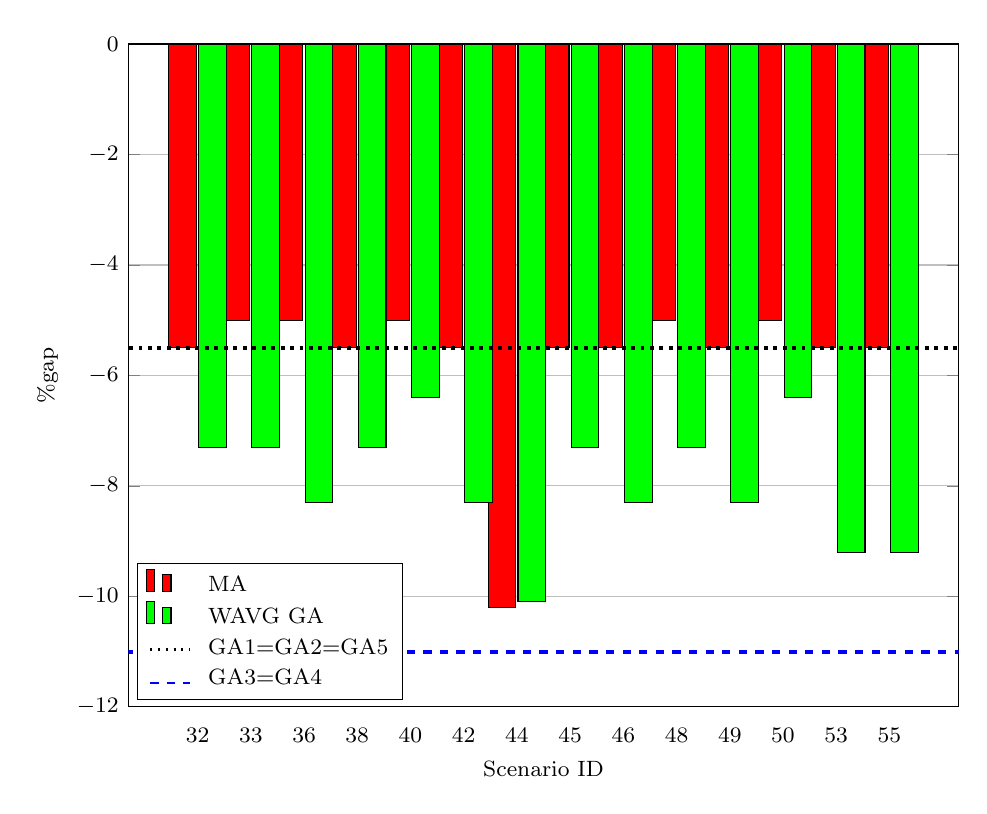
\begin{tikzpicture}[font=\footnotesize,baseline]
		\begin{axis}[
				width  = \textwidth,
				height = 10cm,
				major x tick style = transparent,
				ybar=2*\pgflinewidth,
				bar width=10pt,
				ymajorgrids = true,
				ymin=-12,
				ymax=0,
                xlabel = {Scenario ID },
				ylabel = {\%gap},
                symbolic x coords={32,33,36,38,40,42,44,45,46,48,49,50,53,55},
				xtick = data,
				scaled y ticks = false,
				enlarge x limits=0.10,
				legend cell align=left,
				legend entries={MA, WAVG GA, GA1=GA2=GA5, GA3=GA4},
				legend style={
					at={(0.01,0.01)},
					anchor=south west,
					column sep=1ex
				}
			]
            \addplot[color=black, fill=red,mark=none] coordinates {(32,-5.5)(33,-5.0)(36,-5.0)(38,-5.5)(40,-5.0)(42,-5.5)(44,-10.2)(45,-5.5)(46,-5.5)(48,-5.0)(49,-5.5)(50,-5.0)(53,-5.5)(55,-5.5)};
            \addplot[color=black,fill=green,mark=none] coordinates {(32,-7.3 )(33,-7.3 )(36,-8.3 )(38,-7.3 )(40,-6.4 )(42,-8.3 )(44,-10.1 )(45,-7.3 )(46,-8.3 )(48,-7.3 )(49,-8.3 )(50,-6.4 )(53,-9.2 )(55,-9.2 )};
            \draw[dotted,thick,black,line width = 0.5mm] (-20,65) -- (200,65);
            \draw[dashed,thick,blue,line width = 0.5mm] (-20,10) -- (200,10); 
            \legend{MA, WAVG GA}
            \addlegendimage{my legend}
            \addlegendentry{GA1=GA2=GA5}
            \addlegendimage{my legend2}
            \addlegendentry{GA3=GA4}
		\end{axis}
	\end{tikzpicture}
	\caption{Effect of heterogeneity}

	\label{fig:HeterogeneityAnalysis}
\end{figure}


 
The results obtained clearly demonstrate the significant impact of the operator \replaced[comment]{ behavior }{ behaviour } on the productivity of a production system, even if it is a relatively straightforward system producing a single type of product in a  \replaced[comment]{ dual-resource-constrained }{ dual-resource constrained } flow-shop production system. The findings underscore the importance of recognizing the role of human factors in manufacturing processes and highlight the need for targeted interventions to optimize performance. These insights have broader implications for enhancing productivity and efficiency in a variety of industrial settings.
				   
					
					
\begin{longtable}{|c|c|c|c|c|c|c|c|c|r|c|}
	\hline
	& & \multicolumn{2}{c|}{Inputs} & \multicolumn{3}{c|}{Optimal assignment} & \multicolumn{2}{c|}{Worst assignment }& \multicolumn{2}{c|}{}\\
	&  & Profiles & Mixprod & \multicolumn{3}{c|}{} & \multicolumn{2}{c|}{} & \multicolumn{2}{c|}{}\\
    \it{GR} & \it{ID} & \multicolumn{1}{c|}{$(n_0,..,n_5)$} & \multicolumn{1}{c|}{$(I_1,..,I_3)$} & {$(a^*_1,..,a^*_6)$} & \it{obj}$^*$ & $(q^*_1$,...,$q^*_3)$ & {$(a^{\textsc{w}}_1,..,a^{\textsc{w}}_6)$} & \it{obj}$^{\textsc{w}}$ & \it{\%gap}   & \it{ cpu [min]} \\								
	\hline 
									
	                   & 56      & 1,1,1,1,1,1                         & 1,0,0                               & 4,2,3,0,1,5          & 536          & 536,0,0               & 1,4,5,3,0,2                                & 493                     & 8.0     & 13.2   \\
	                   & 57      & 1,1,1,1,1,1                         & 0,1,0                               & 1,0,3,4,2,5          & 565          & 0,565,0               & 1,4,5,3,0,2                                & 536                     & 5.0 & 13.6  \\
	                   & 58      & 1,1,1,1,1,1                         & 0,0,1                               & 3,0,5,2,4,1          & 661          & 0,0,661               & 1,4,5,3,0,2                                & 651                     & 1.4    & 13.9 \\
	{GH}\label{SEN:GH} & 59      & 1,1,1,1,1,1                         & 1,1,0                               & 4,0,3,2,1,5          & 579          & 24,555,0               & 1,4,5,3,0,2                                & 550                     & 4.9    & 13.3     \\
	                   & 60      & 1,1,1,1,1,1                         & 1,0,1                               & 4,0,3,1,2,5          & 661          & 5,0,656               & 1,4,5,3,0,2                                & 651                     & 1.4   & 13.7      \\
	                   & 61      & 1,1,1,1,1,1                         & 0,1,1                               & 3,0,4,2,5,1          & 680          & 0,168,512              & 1,4,5,3,0,2                                & 665                     & 2.1      & 13.9  \\
	                   & 62      & 1,1,1,1,1,1                         & 1,1,1                               & 1,4,3,0,2,5          & 704          & 34,86,584              & 1,4,5,3,0,2                                & 675                     & 4.0    & 13.7     \\						        
	\hline
	\caption{Results of the GH scenario group} 
	\label{tab:tr4}
\end{longtable}
			
					

				
The aim of the last scenario group (GH) is to test the efficiency of the proposed model when several product types are considered. In this situation, the optimization model will determine the best assignment of workers,  the amount of production for each product type, and the scheduling of all product operations in order to Maximize production throughput.\deleted[]{ Due to the complexity of the problem, we reduced the optimization horizon from one week to one day.} We also considered several product mixes (ProdMix), as shown in Table~\ref{tab:tr4}. We notice that Mixprod has a significant impact on optimal assignment and productivity. 
			
After \replaced[]{analyzing }{ analysing } scenarios 56, 57, and 58, it is clear that selecting type 3 of the product leads to the highest throughput. This is mainly due to its better workstation balancing, which results in a shorter cycle time of only 3-time units. Although type 3 has the longest total processing time of 16-time units, it more than compensates for it with its other advantages, making it the optimal choice to achieve maximum throughput.  
		
Scenarios 59, 60, and 61 propose the production of two types of products with minimal production (production mix) of one part $q_t^{min}= 1$. When comparing scenario 59 (selection of product types 1 and 2) with scenarios 56 (product type 1) and 57 (product type 2), it is clear that the productivity of scenario 59 has been improved due to the scheduling of jobs by product type. However, the optimal solution generates 5 products of type 1 and 116 of product type 2 due to the reduced total processing time of the type 2 product (15-time \replaced[]{ units }{ unit } for type 1 VS 11 time \replaced[]{ units }{ unit } for type 2) and the same nominal cycle time of 4- time units. 
			
			
In Scenario 60, we observe that the optimal solution involves producing 137 units of type 3 and only one unit of type 1. Conversely, scenario 58 revealed that the optimal solution includes 138 units of type 1. This indicates that the production of type 1 product is not ideal for \replaced[comment]{ maximizing }{ maximising } throughput and is instead only necessary due to the constraint outlined in (\ref{c7}), which requires the production of at least one unit of type 1 product to be produced.
The maximum throughput corresponds to scenario 62 (with an optimal throughput of 147), where all types of products are selected. This allows us to conclude that productivity increases as we have \replaced[]{ many }{ a large number of }{} product types. 
The optimal assignment of the worker profile tray is to increase the balance of the production line based on the punctuality of the profiles. For example, in scenario 56, the best profiles are assigned to the worst \replaced[comment]{ workstations}{ machines }, which increases the balancing of the lines and increases the production system throughput. 
	
						       
					
\section{Managerial insights }\label{sec:mins}



This study \replaced[]{ emphasizes }{ emphasises }{} the critical role of effective human resource allocation strategies in achieving maximum throughput in manufacturing environments. Assignment of the best worker profiles to bottleneck workstations is particularly mandatory for success. The largest gaps between the best and worst allocation strategies are observed when multiple perfect profiles are available, highlighting the importance of such strategies. The problem becomes more complex when it is not easy to define the bottleneck \replaced[comment]{ workstation }{ machine } due to the production of different types of products with different processing times.  
The study also underscores the significant impact of operator \replaced[comment]{ behavior }{ behaviour } on productivity in a production system, highlighting the need to \replaced[]{ recognize }{ recognise }{} human factors and implement targeted interventions for optimal performance. These insights can help improve productivity and efficiency in various industrial settings. Additionally, the study demonstrates that the selection of the right product type is essential to optimize the efficiency of an optimization model to \replaced[]{ maximize }{ maximise } production throughput. Choosing the product with the \replaced[]{ shortest }{ smallest }{}  nominal cycle time \added[]{in the production mix} resulted in the highest throughput despite having \replaced[]{other products with longer nominal cycle times.}{a longer total processing time due to better balancing of the workstation}. Furthermore, a larger number of product types can increase productivity, and optimizing the assignment of worker profiles can improve line balancing and further increase production system throughput.\added[comment=$R1^{10}$]{ Considering the inclusion and skill development of workers is a crucial aspect of tactical decision-making, which can be facilitated through team rotation and varying the production mix. We believe that implementing our algorithm can create a more inclusive environment where individuals with profiles unsuitable for a particular workstation can be automatically reassigned to another workstation where they can effectively contribute to production.} 

\added[comment=$R1^{15}$]{Moreover, this solution enables the use of all available profiles, considering current levels of skills and motivations. The ability to test various scenarios representing different combinations of profiles provides an effective tool for human resources managers to define their strategies for shits/crew planning, recruiting, training, and skills enhancement. This holistic approach to workforce management ensures that the right individuals are assigned to the right tasks at the right time, optimizing overall productivity and performance.}

Finally, the study highlights the importance of selecting mixed-team workers, particularly in manufacturing systems with a high mix of production.  

Indeed, the results obtained from this study suggest that the consideration of teams with heterogeneous profiles, combined with optimized assignment strategies, tends to be more beneficial than relying on homogeneous teams evolving over time. The worker \replaced[comment]{ behavior }{ behaviour } based on stochastic modeling of the punctuality can be obtained from the record of operator actions and movements, which constitutes an objective and factual measure. This behavior model based on punctuality can be considered a symptom revealer of other hidden aspects, such as the operator's well-being, the workstation's adaptation to the worker, and the level of fatigue. Our research is driven by the human-centered approach to production planning, which seeks to tailor scheduling and task allocation to each worker's unique profile. By considering these individual factors, managers can unlock significant improvements in workforce productivity. 

While the manager may not be able to determine the exact dynamic effect of one worker on another, assigning a specific worker with a particular behavior will still influence the assignment of other workers, whether they have equivalent or different behaviors and skills. 

					
\section{Conclusions and future works  }\label{sec:conc3}  
This work presents an approach for \replaced[]{ modeling}{ modelling }{}, simulating and optimizing the impact of human \replaced[comment]{ behavior }{ behaviour } on production throughput. A stochastic approach to model human \replaced[comment]{ behavior }{ behaviour } in terms of punctuality on the workstation is proposed and simulated in a dual resource flow-shop production system. A non-linear optimization model is proposed to provide the optimal assignment of workers to \replaced[comment]{ workstations}{ machines }, the optimal scheduling of production operations, and the optimal mix of production to maximize production throughput, while considering the possibility of operations interruption. The results show that human \replaced[comment]{ behavior }{ behaviour } has an important influence on the productivity of the production system, especially when the number of product and worker profiles increases. The analyses of results demonstrate the complexity of selecting the best worker profile for the best \replaced[comment]{ workstation}{ machine }. especially in high-mix production systems. In \replaced[comment]{ dual-resource-constrained }{ dual-resource constrained } flow-shop production system, it is very important to ensure a good balance of the production line, and the assignment of human workers plays an important role in \replaced[comment]{ maximizing }{ maximising } the throughput of the production system.

By modeling human behavior and developing predictive models of worker performance and \replaced[comment]{ behavior}{ behaviour }, production planning can be optimized while taking into account the unique characteristics of each individual or a similar group (profile). This personalized approach has the potential to significantly enhance the overall productivity of the workforce. In this work, we demonstrate that punctuality, as a subtle indicator of a worker's hidden aspects, significantly impacts production and performance metrics such as effective processing time and overall productivity. In particular, the frequent breaks taken by an operator may be an underlying symptom of factors such as fatigue, well-being, or motivation. 

One of the limits of the proposed optimization model is that it takes into account only one aspect affected by human \replaced[comment]{ behavior }{ behaviour } and a single objective, which is the maximization of the throughput. Moreover, it does not consider the possible evolution of operators' behavioral profiles during the production planning horizon or dependently on the workstation and does not consider the interaction between operators that can lead to the unexpected group \replaced[]{ behavior }{ behaviour }{}. All these considerations represent a potential future work that can be addressed.

In the next step, we plan to improve our human \replaced[comment]{ behavior }{ behaviour } models by incorporating factors such as experience, skills, and personality to improve the accuracy of the proposed optimization model.
Moreover, it will be worthwhile to develop approximate methods (e.g., meta-heuristics) to solve the proposed optimization model in order to be able to handle more realistic cases in terms of instance size.
Another interesting perspective of this work involves the evolution of behavior through the improvement of skill levels and the impact of one worker on another within the same team.
% \textcolor{red}{   talking about the consideration of the interaction between operators in a single team. }
To validate our theoretical results, we will apply our approach to a real-world case study and observe the impact of optimal worker \replaced[comment]{ behavior }{ behaviour } on system performance in a dynamic environment. This will not only help validate our approach but also provide valuable data for predicting worker states and integrating that information into an adaptive decision-making process for worker assignment and production task scheduling. The development of such realistic cases will also allow for observing phenomena such as group behavior and variation in human profiles and testing and validating new data collection and dynamic decision-making technologies.
Our ultimate goal is to develop a robust and effective optimization model that considers the human factor in manufacturing processes to improve productivity and efficiency while improving human well-being in a manufacturing environment.
	
%\section*{Acknowledgment}\label{sec:Acknow}
%Acknowledgement is made to the Normandy region and the European Union for supporting this research through the RIN regional research programme by funding the AntiHpert project.

%% If you have bibdatabase file and want bibtex to generate the
%% bibitems, please use
%%
% \listoffigures
% \listoftables
%\newpage
%\thispagestyle{empty}
%\bibliographystyle{elsarticle-num} 
% \bibliographystyle{elsarticle-num-names} 
 %\bibliography{cas-refs2}

\begin{thebibliography}{10}
	\expandafter\ifx\csname url\endcsname\relax
	\def\url#1{\texttt{#1}}\fi
	\expandafter\ifx\csname urlprefix\endcsname\relax\def\urlprefix{URL }\fi
	\expandafter\ifx\csname href\endcsname\relax
	\def\href#1#2{#2} \def\path#1{#1}\fi
	
	\bibitem{lyngstadaas2022harder}
	H.~Lyngstadaas, T.~Berg, Harder, better, faster, stronger: digitalisation and
	employee well-being in the operations workforce, Production Planning \&
	Control (2022) 1--18.
	
	\bibitem{fantini2020placing}
	P.~Fantini, M.~Pinzone, M.~Taisch, Placing the operator at the centre of
	industry 4.0 design: Modelling and assessing human activities within
	cyber-physical systems, Computers \& Industrial Engineering 139 (2020)
	105058.
	
	\bibitem{pinzone2020framework}
	M.~Pinzone, F.~Alb{\`e}, D.~Orlandelli, I.~Barletta, C.~Berlin, B.~Johansson,
	M.~Taisch, A framework for operative and social sustainability
	functionalities in human-centric cyber-physical production systems, Computers
	\& industrial engineering 139 (2020) 105132.
	
	\bibitem{raja2023industry}
	A.~Raja~Santhi, P.~Muthuswamy, Industry 5.0 or industry 4.0 s? introduction to
	industry 4.0 and a peek into the prospective industry 5.0 technologies,
	International Journal on Interactive Design and Manufacturing (IJIDeM) (2023)
	1--33.
	
	\bibitem{messaadia2016plm}
	M.~Messaadia, D.~Baudry, A.~Louis, S.~Mahdikhah, R.~Evans, J.~Gao, T.~Paquet,
	M.~Sahnoun, B.~Mazari, {PLM} adoption in {SME}s context, Computer-Aided
	Design and Applications 13~(5) (2016) 618--627.
	
	\bibitem{brik2022fog}
	B.~Brik, M.~Messaadia, M.~Sahnoun, B.~Bettayeb, M.~A. Benatia, Fog-supported
	low latency monitoring of system disruptions in industry 4.0: A federated
	learning approach, ACM Transactions on Cyber-Physical Systems (2022).
	
	\bibitem{kadir2020human}
	B.~A. Kadir, O.~Broberg, Human well-being and system performance in the
	transition to industry 4.0, International Journal of Industrial Ergonomics 76
	(2020) 102936.
	
	\bibitem{bailly2020}
	A.~Bailly, H.~Tlahig, B.~Bettayeb, M.~Messaadia, M.~Sahnoun, Human’s new
	roles to ensure resilience of industrial cyber-physical systems, in: 2020
	IEEE Conference on Industrial Cyberphysical Systems (ICPS), Vol.~1, IEEE,
	2020, pp. 453--458.
	
	\bibitem{chen2022analysis}
	N.~Chen, N.~Huang, R.~Radwin, J.~Li, Analysis of assembly-time performance
	(atp) in manufacturing operations with collaborative robots: a systems
	approach, International Journal of Production Research 60~(1) (2022)
	277--296.
	
	\bibitem{kose2023game}
	Y.~Kose, E.~Cevikcan, S.~Ertemel, M.~Murat, Game theory-oriented approach for
	disassembly line worker assignment and balancing problem with multi-manned
	workstations, Computers \& Industrial Engineering 181 (2023) 109294.
	
	\bibitem{dolgui2022design}
	A.~Dolgui, F.~Sgarbossa, M.~Simonetto, Design and management of assembly
	systems 4.0: systematic literature review and research agenda, International
	Journal of Production Research 60~(1) (2022) 184--210.
	
	\bibitem{Jamal2019Work}
	A.~Jamal, Work turnover and its impact on the quality of productivity in the
	industrial sector, Research in World Economy 10 (2019) 65.
	\newblock \href {https://doi.org/10.5430/rwe.v10n4p65}
	{\path{doi:10.5430/rwe.v10n4p65}}.
	
	\bibitem{Acar2018Creativity}
	O.~A. Acar, M.~Tarakci, D.~van Knippenberg, Creativity and innovation under
	constraints: A cross-disciplinary integrative review, Journal of Management
	45 (2018) 121 -- 96.
	\newblock \href {https://doi.org/10.1177/0149206318805832}
	{\path{doi:10.1177/0149206318805832}}.
	
	\bibitem{Destouet2023}
	C.~Destouet, H.~Tlahig, B.~Bettayeb, B.~Mazari, Flexible job shop scheduling
	problem under industry 5.0: A survey on human reintegration, environmental
	consideration and resilience improvement, Journal of Manufacturing Systems 67
	(2023) 155--173.
	
	\bibitem{battini2022towards}
	D.~Battini, N.~Berti, S.~Finco, I.~Zennaro, A.~Das, Towards industry 5.0: A
	multi-objective job rotation model for an inclusive workforce, International
	Journal of Production Economics 250 (2022) 108619.
	
	\bibitem{missimer2017strategic}
	M.~Missimer, K.-H. Rob{\`e}rt, G.~Broman, A strategic approach to social
	sustainability--part 1: exploring the social system, Journal of cleaner
	production 140 (2017) 32--41.
	
	\bibitem{trost2022social}
	M.~Trost, T.~Claus, F.~Herrmann, Social sustainability in production planning:
	A systematic literature review, Sustainability 14~(13) (2022) 8198.
	
	\bibitem{panagou2023scoping}
	S.~Panagou, W.~P. Neumann, F.~Fruggiero, A scoping review of human robot
	interaction research towards industry 5.0 human-centric workplaces,
	International Journal of Production Research (2023) 1--17.
	
	\bibitem{zanchettin2018}
	A.~M. Zanchettin, A.~Casalino, L.~Piroddi, P.~Rocco, Prediction of human
	activity patterns for human--robot collaborative assembly tasks, IEEE
	Transactions on Industrial Informatics 15~(7) (2018) 3934--3942.
	
	\bibitem{zhang2021task}
	M.~Zhang, C.~Li, Y.~Shang, H.~Huang, W.~Zhu, Y.~Liu, A task scheduling model
	integrating micro-breaks for optimisation of job-cycle time in human-robot
	collaborative assembly cells, International Journal of Production Research
	(2021) 1--12.
	
	\bibitem{hjorth2022human}
	S.~Hjorth, D.~Chrysostomou, Human--robot collaboration in industrial
	environments: A literature review on non-destructive disassembly, Robotics
	and Computer-Integrated Manufacturing 73 (2022) 102208.
	
	\bibitem{liu2022application}
	L.~Liu, F.~Guo, Z.~Zou, V.~G. Duffy, Application, development and future
	opportunities of collaborative robots (cobots) in manufacturing: A literature
	review, International Journal of Human--Computer Interaction (2022) 1--18.
	
	\bibitem{vicentini2021collaborative}
	F.~Vicentini, Collaborative robotics: a survey, Journal of Mechanical Design
	143~(4) (2021).
	
	\bibitem{hentout2019human}
	A.~Hentout, M.~Aouache, A.~Maoudj, I.~Akli, Human--robot interaction in
	industrial collaborative robotics: a literature review of the decade
	2008--2017, Advanced Robotics 33~(15-16) (2019) 764--799.
	
	\bibitem{Jahanmahin2022}
	R.~Jahanmahin, S.~Masoud, J.~Rickli, A.~Djuric, Human-robot interactions in
	manufacturing: {A} survey of human behavior modeling, Robotics and
	Computer-Integrated Manufacturing 78 (2022) 102404.
	
	\bibitem{ferjani2015}
	A.~Ferjani, A.~Ammar, H.~Pierreval, A.~Trabelsi, F.~Aubi{\`e}re, A heuristic
	approach taking operators’ fatigue into account for the dynamic assignment
	of workforce to reduce the mean flowtime, in: International Conference on
	Computers and Industrial Engineering, CIE45, Vol.~43, 2015, pp. 65--80.
	
	\bibitem{ferjani2017}
	A.~Ferjani, A.~Ammar, H.~Pierreval, S.~Elkosantini, A simulation-optimization
	based heuristic for the online assignment of multi-skilled workers subjected
	to fatigue in manufacturing systems, Computers \& Industrial Engineering 112
	(2017) 663--674.
	
	\bibitem{Berlin2017}
	C.~Berlin, C.~Adams, Production ergonomics: Designing work systems to support
	optimal human performance, Ubiquity press, 2017.
	
	\bibitem{Greig2019}
	M.~Greig, J.~Village, S.~Dixon, F.~Salustri, W.~Neumann, Assessing human
	factors and ergonomics capability in organizations - {The} {Human} {Factors}
	{Integration} {Toolset}, Ergonomics 62 (2019) 1--30.
	
	\bibitem{Azarkhil2014}
	M.~Azarkhil, A.~Mosleh, Dynamic behavior of operating crew in complex systems,
	in: 2014 {Reliability} and {Maintainability} {Symposium}, 2014, pp. 1--7,
	iSSN: 0149-144X.
	
	\bibitem{DiPasquale2013}
	V.~Di~Pasquale, R.~Iannone, S.~Miranda, S.~Riemma, et~al., An overview of human
	reliability analysis techniques in manufacturing operations, in: Operations
	Management, Vol.~9, chapter, 2013, pp. 978--953.
	
	\bibitem{Dantan2020}
	J.-Y. Dantan, A.~Etienne, J.~Petronijevic, A.~Siadat, Tolerance \& {Time}
	margin, Procedia CIRP 92 (2020) 51--56.
	
	\bibitem{Upadhyay2022}
	R.~K. Upadhyay, A.~Singh, B.~M. Singh, Human side of cybersecurity: an
	empirical study, International Journal of Business Information Systems 41~(3)
	(2022) 408--422.
	
	\bibitem{SanchezAguayo2021}
	M.~S{\'a}nchez-Aguayo, L.~Urquiza-Aguiar, J.~Estrada-Jim{\'e}nez, Fraud
	detection using the fraud triangle theory and data mining techniques: {A}
	literature review, Computers 10~(10) (2021).
	
	\bibitem{Domarkiene2021}
	I.~Domarkienė, L.~Ambrozaitytė, L.~Bukauskas, T.~Rančelis, S.~Sütterlin,
	B.~Knox, K.~Maennel, O.~Maennel, K.~Parish, R.~Lugo, A.~Brilingaitė,
	Cybergenomics: {Application} of behavioral genetics in cybersecurity,
	Behavioral Sciences 11~(11) (2021).
	
	\bibitem{Moallem2021}
	A.~Moallem, Cybersecurity, privacy, and trust, in: Handbook of Computer
	Networks and Cyber Security, Wiley Online Library, 2021, pp. 1107--1120.
	
	\bibitem{Schia2019}
	M.~H. Schia, The introduction of AI in the construction industry and its impact
	on human behavior, NTNU, 2019.
	
	\bibitem{Kong2020}
	F.~S. Kong, X.~D. Kong, H.~Y. Wu, Y.~X. Zhang, P.~D. Fang, Simulation
	{Modeling} of {Production} {System} {Considering} {Human} {Behavior}, in:
	2020 {IEEE} {International} {Conference} on {Industrial} {Engineering} and
	{Engineering} {Management} ({IEEM}), 2020, pp. 123--127.
	
	\bibitem{Mossa2015}
	G.~Mossa, F.~Boenzi, S.~Digiesi, G.~Mummolo, V.~A. Romano, {Productivity and
		ergonomic risk in human based production systems: A job-rotation scheduling
		model}, International Journal of Production Economics 171 (2016) 471--477.
	
	\bibitem{Katiraee2021a}
	N.~Katiraee, M.~Calzavara, S.~Finco, D.~Battini, O.~Battaïa, Consideration of
	workers’ differences in production systems modelling and design {State} of
	the art and directions for future research, International Journal of
	Production Research 59 (Mar. 2021).
	
	\bibitem{ayough2023robust}
	A.~Ayough, B.~Khorshidvand, Robust optimization for the integrated worker-cell
	assignment and sequencing problem in a lean u-shaped assembly line, Computers
	\& Industrial Engineering 178 (2023) 109139.
	
	\bibitem{Bouaziz2022}
	N.~Bouaziz, B.~Bettayeb, M.~Sahnoun, A.~Yassine, A.~Latreche, Modeling and
	simulation of human behavior impact on production throughput,
	IFAC-PapersOnLine 55 (2022) 1740--1745.
	
	\bibitem{dhiflaoui2018dual}
	M.~Dhiflaoui, H.~E. Nouri, O.~B. Driss, Dual-resource constraints in classical
	and flexible job shop problems: a state-of-the-art review, Procedia computer
	science 126 (2018) 1507--1515.
	
	\bibitem{geurtsen2023production}
	M.~Geurtsen, J.~B. Didden, J.~Adan, Z.~Atan, I.~Adan, Production, maintenance
	and resource scheduling: A review, European Journal of Operational Research
	305~(2) (2023) 501--529.
	
	\bibitem{hashemi2020operations}
	S.~E. Hashemi-Petroodi, S.~Thevenin, S.~Kovalev, A.~Dolgui, Operations
	management issues in design and control of hybrid human-robot collaborative
	manufacturing systems: a survey, Annual Reviews in Control 49 (2020)
	264--276.
	
	\bibitem{Bogataj2018}
	D.~Bogataj, D.~Battini, M.~Calzavara, A.~Persona, {The ageing workforce
		challenge: Investments in collaborative robots or contribution to pension
		schemes, from the multi-echelon perspective}, International Journal of
	Production Economics 210 (2019) 97--106.
	
	\bibitem{Onay2023}
	A.~Onay, C.~Stampfer, H.~Missbauer, {A behavioral perspective on workload
		control concepts: The influence of order release on operators' reaction
		behavior}, International Journal of Production Economics 264~(May) (2023)
	108956.
	
	\bibitem{Bentefouet2012}
	F.~Bentefouet, D.~A. Nembhard, {Optimal flow-line conditions with worker
		variability}, International Journal of Production Economics 141~(2) (2013)
	675--684.
	
	\bibitem{lucchese2023stochastic}
	A.~Lucchese, S.~Digiesi, G.~Mummolo, A stochastic-based model to assess the
	variability of task completion times of differently aged and experienced
	workers subject to fatigue, in: IFIP International Conference on Advances in
	Production Management Systems, Springer, 2023, pp. 745--759.
	
	\bibitem{lin2022human}
	C.-H. Lin, K.-J. Wang, A.~A. Tadesse, B.~H. Woldegiorgis, Human-robot
	collaboration empowered by hidden semi-markov model for operator behaviour
	prediction in a smart assembly system, Journal of Manufacturing Systems 62
	(2022) 317--333.
	
	\bibitem{vijayakumar2022framework}
	V.~Vijayakumar, F.~Sgarbossa, W.~P. Neumann, A.~Sobhani, Framework for
	incorporating human factors into production and logistics systems,
	International Journal of Production Research 60~(2) (2022) 402--419.
	
	\bibitem{elkosantini2009integration}
	S.~Elkosantini, D.~Gien, Integration of human behavioural aspects in a dynamic
	model for a manufacturing system, International Journal of Production
	Research 47~(10) (2009) 2601--2623.
	
	\bibitem{chang2008synthesized}
	W.-L. Chang, S.-T. Yuan, A synthesized model of markov chain and {ERG} theory
	for behavior forecast in collaborative prototyping, Journal of Information
	Technology Theory and Application (JITTA) 9~(2) (2008) 5.
	
	\bibitem{Digiesi2009}
	S.~Digiesi, A.~A. Kock, G.~Mummolo, J.~E. Rooda, {The effect of dynamic worker
		behavior on flow line performance}, International Journal of Production
	Economics 120~(2) (2009) 368--377.
	
	\bibitem{BERTI2021108151}
	N.~Berti, S.~Finco, O.~Battaïa, X.~Delorme, Ageing workforce effects in
	dual-resource constrained job-shop scheduling, International Journal of
	Production Economics 237 (2021) 108151.
	
	\bibitem{digiesi2020human}
	S.~Digiesi, D.~Cavallo, A.~Lucchese, C.~Mummolo, Human cognitive and motor
	abilities in the aging workforce: An information-based model, Applied
	Sciences 10~(17) (2020) 5958.
	
	\bibitem{korytkowski2017competences}
	P.~Korytkowski, Competences-based performance model of multi-skilled workers
	with learning and forgetting, Expert Systems with applications 77 (2017)
	226--235.
	
	\bibitem{Al-E-Hashem2009}
	S.~M. J.~M. Al-E-Hashem, M.~B. Aryanezhad, V.~Deljoo, S.~M. J.~M. Al, Dynamic
	cell formation and the worker assignment problem: a new model, Springer 41
	(2009) 329--342.
	
	\bibitem{Chu2019}
	X.~Chu, D.~Gao, S.~Cheng, L.~Wu, J.~Chen, Y.~Shi, Q.~Qin, Worker assignment
	with learning-forgetting effect in cellular manufacturing system using
	adaptive memetic differential search algorithm, Computers \& industrial
	engineering 136 (2019) 381--396.
	
	\bibitem{green2017hybrid}
	J.~J. Green, C.~C. Krejci, D.~E. Cantor, A hybrid simulation model of helping
	behavior, in: 2017 Winter Simulation Conference (WSC), IEEE, 2017, pp.
	1619--1630.
	
	\bibitem{Mura2019a}
	M.~Dalle~Mura, G.~Dini, Designing assembly lines with humans and collaborative
	robots: A genetic approach, CIRP Annals 68~(1) (2019) 1--4.
	
	\bibitem{Mura2019b}
	M.~Dalle~Mura, G.~Dini, Optimizing ergonomics in assembly lines: A multi
	objective genetic algorithm, CIRP Journal of Manufacturing Science and
	Technology 27 (2019) 31--45.
	
	\bibitem{Ramezanian2015}
	R.~Ramezanian, A.~Ezzatpanah, Modeling and solving multi-objective mixed-model
	assembly line balancing and worker assignment problem, Computers \&
	Industrial Engineering 87 (2015) 74--80.
	
	\bibitem{Liu2019}
	M.~Liu, X.~Yang, Bi-objective optimization for scheduling and multi-skilled
	worker assignments in the hybrid flow shop, IFAC-PapersOnLine 52 (2019)
	2128--2133.
	
	\bibitem{Chen2019a}
	J.~C. Chen, Y.-Y. Chen, T.-L. Chen, Y.-H. Kuo, Applying two-phase adaptive
	genetic algorithm to solve multi-model assembly line balancing problems in
	tft--lcd module process, Journal of Manufacturing Systems 52 (2019) 86--99.
	
	\bibitem{Katiraee2022}
	N.~Katiraee, M.~Calzavara, S.~Finco, O.~Batta{\"\i}a, D.~Battini, Assembly line
	balancing and worker assignment considering workers’ expertise and
	perceived physical effort, International Journal of Production Research
	(2022) 1--21.
	
	\bibitem{Wu2018a}
	L.~Wu, F.~Cai, L.~Li, X.~Chu, Cross-trained worker assignment problem in
	cellular manufacturing system using swarm intelligence metaheuristics,
	Mathematical Problems in Engineering 2018 (2018) 1--15.
	
	\bibitem{Zacharia2015}
	M.~Peron, S.~Arena, G.~J.~L. Micheli, F.~Sgarbossa, A decision support system
	for designing win--win interventions impacting occupational safety and
	operational performance in ageing workforce contexts, Safety science 147
	(2022) 105598.
	
	\bibitem{Borba2013}
	L.~Borba, M.~Ritt, A heuristic and a branch-and-bound algorithm for the
	assembly line worker assignment and balancing problem, Computers \&
	Operations Research 45 (2014) 87--96.
	
	\bibitem{Vila2014}
	M.~Vilà, J.~Pereira, A branch-and-bound algorithm for assembly line worker
	assignment and balancing problems, Computers and Operations Research 44
	(2014) 105--114.
	
	\bibitem{Moussavi2017}
	S.~E. Moussavi, M.~Mahdjoub, O.~Grunder, Productivity improvement through a
	sequencing generalised assignment in an assembly line system, International
	Journal of Production Research 55 (2017) 7509--7523.
	
	\bibitem{LUO2023102534}
	Q.~Luo, Q.~Deng, G.~Xie, G.~Gong, A pareto-based two-stage evolutionary
	algorithm for flexible job shop scheduling problem with worker cooperation
	flexibility, Robotics and Computer-Integrated Manufacturing 82 (2023) 102534.
	
	\bibitem{li2023integrating}
	Y.~Li, X.~Chen, Y.~An, Z.~Zhao, H.~Cao, J.~Jiang, Integrating machine layout,
	transporter allocation and worker assignment into job-shop scheduling solved
	by an improved non-dominated sorting genetic algorithm, Computers \&
	Industrial Engineering 179 (2023) 109169.
	
	\bibitem{Lundstrom2016}
	J.~Lundström, E.~Järpe, A.~Verikas, Detecting and exploring deviating
	behaviour of smart home residents, Expert Systems with Applications 55 (2016)
	429--440.
	
	\bibitem{Sanchez2020}
	V.~G. Sánchez, O.~M. Lysaker, N.-O.~O. Skeie, Human behaviour modelling for
	welfare technology using hidden markov models, Pattern Recognition Letters
	137 (2020) 71--79.
	
	\bibitem{costa2020solving}
	A.~Costa, V.~Fernandez-Viagas, J.~M. Frami{\~n}an, Solving the hybrid flow shop
	scheduling problem with limited human resource constraint, Computers \&
	Industrial Engineering 146 (2020) 106545.
	
\end{thebibliography}



% \begin{thebibliography}{00}
% 
\end{document}
\endinput
%%
%% End of file `elsarticle-template-num.tex'.
